%% ------------------------------------------------------------------------- %%
\chapter{Fundamentação Teórica}
\label{cap:conceitos}

%% ------------------------------------------------------------------------- %%
\section{Modelos de cores}\index{cores!modelos de}
\label{sec:fundamentos}

O uso de imagens coloridas em visão computacional ou no processamento de imagens pode ser motivado por dois fatores principais. O primeiro diz respeito a característica poderosa da cor de funcionar como um descritor que, frequentemente, simplifica a identificação e extração de um objeto em uma cena. O segundo está relacionado com a capacidade dos seres humanos de discernir milhares de tonalidades e intensidades, se comparado com apenas algumas dúzias de níveis de cinza \citep{gonzalez:02}.

A percepção visual da cor pelo olho humano não deve variar conforme a distribuição espectral da luz natural incidente sobre um objeto. Em outras palavras, a aparência de cor dos objetos permanece estável sob condições de iluminação diferentes. Esse fenômeno é conhecido como constância de cor \citep{gevers:12}.

Como exemplo, o gramado de um estádio de futebol permanece verde durante todo o dia, inclusive ao entardecer quando, de um ponto de vista físico, a luz solar
tem um aspecto mais avermelhado.

A percepção humana das cores se dá pela ativação de células nervosas que enviam
mensagens ao cérebro sobre brilho (\textit{brightness}), matiz (\textit{hue}) e 
saturação (\textit{saturation}) que, geralmente, são as características usadas
para distinguir uma cor de outra \citep{gonzalez:02}.

O brilho dá a noção de intensidade cromática. Matiz representa a cor dominante
percebida por um observador. Já a saturação refere-se à pureza relativa ou quantidade de luz branca aplicada ao matiz. Combinados, matiz e saturação são conhecidos como cromaticidade e, portanto, uma cor deve ser caracterizada por seu brilho e cromaticidade \citep{gonzalez:02}.

As cores podem ser especificadas por modelos matemáticos em tuplas de números em um sistema de coordenadas e um subespaço dentro desse sistema onde cada cor
é representada por um único ponto. Tais modelos são conhecidos como modelo de cores \citep{gonzalez:02}.

Esses modelos podem ser classificados como de dois tipos: os modelos aditivos em que as intensidades das cores primárias são adicionadas para produzir outras cores e subtrativos, onde as cores são geradas subtraindo-se o comprimento da onda dominante da luz branca.

As seções seguintes descrevem brevemente alguns dos principais modelos de cores, bem como seus variantes e principais áreas de aplicação.

%% ------------------------------------------------------------------------- %%
\subsection{Modelo de Munsell}\index{cores!modelo de Munsell}
\label{sec:modelo_cores_munsell}

Pioneiro na tentativa de organizar a percepção de cor em um espaço de cores, Albert H. Munsell conseguiu aliar a arte e a ciência das cores em uma única teoria \citep{konstantinos:00}.

O princípio da igualdade de espaçamento entre os componentes do modelo é a ideia principal do modelo de cores de Munsell \citep{konstantinos:00}. Esses componentes são matiz (\textit{hue}), luminosidade (\textit{value}) e saturação (\textit{chroma}).

O modelo é representado por uma forma cilíndrica e pode ser visto na figura~\ref{fig:munsell-system}. O matiz está disposto no eixo circular que consiste de cinco cores de base e cinco secundárias, a saturação no eixo radial e a luminosidade no eixo vertical em uma escala variando de 0 a 10.

\begin{figure}[!h]
  \centering
  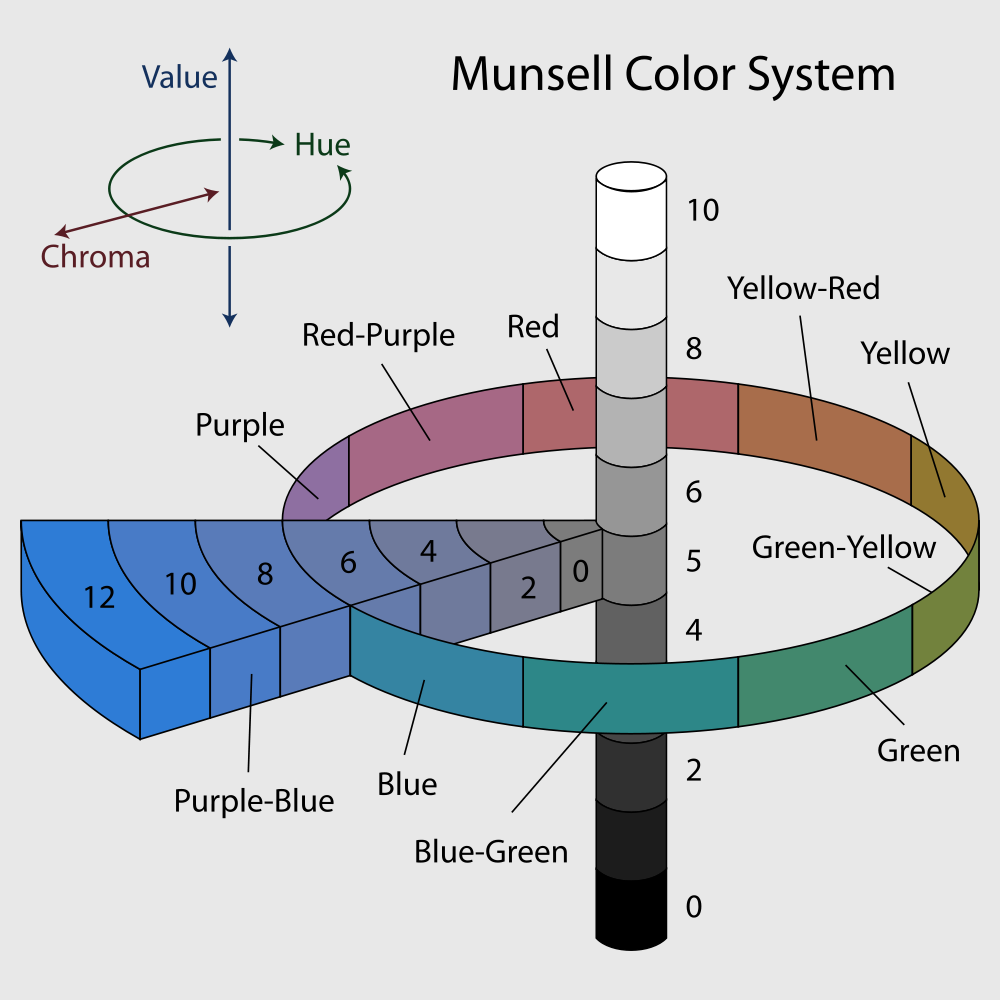
\includegraphics[width=.55\textwidth]{munsell-system}
  % fonte https://commons.wikimedia.org/wiki/File:Munsell-system.svg
  \caption[Modelo de cores de Munsell.]{Modelo de cores de Munsell representado por uma forma cilíndrica. O matiz está disposto no eixo circular que consiste de cinco cores de base e cinco secundárias, a saturação no eixo radial e a luminosidade no eixo vertical em uma escala variando de 0 a 10. Fonte: \citet{rus:07}.}
  \label{fig:munsell-system} 
\end{figure}

%% ------------------------------------------------------------------------- %%
\subsection{Modelo CIE}\index{cores!modelo CIE}
\label{sec:modelo_cores_cie}

Em 1931, o CIE estabeleceu o primeiro modelo matemático de especificação numérica da cor, cujo objetivo era analisar a relação entre os aspectos físicos das cores no espectro eletromagnético e sua percepção pelo sistema visual humano para determinar como uma pessoa comum percebe a cor. Uma revisão desta especificação foi publicada em 1964 \citep{gonzalez:02}.

O experimento que originou o padrão consistia em detectar as cores percebidas por um observador a partir de uma mistura de três cores primárias X, Y e Z chamadas de valores tristímulus. Estas coordenadas deram origem ao espaço de cores \textbf{CIE XYZ} que engloba todas as cores que podem ser percebidas por um ser humano comum e, por esta razão, é considerado uma representação independente de dispositivo \citep{konstantinos:00}.

O sistema proposto pelo CIE XYZ para descrição de uma cor é baseado em um componente de luminância Y e outros dois componentes adicionais X e Z que dão a informação de cromaticidade. Esse sistema é formado por cores imaginárias que podem ser expressas como combinações das medidas normalizadas abaixo:


\begin{equation}
  x = \frac{X}{X + Y + Z}
\end{equation}

\begin{equation}
  y = \frac{Y}{X + Y + Z}
\end{equation}

\begin{equation}
  z = \frac{Z}{X + Y + Z}
\end{equation}

com $x + y+ z = 1$.

As combinações de valores negativos e outros problemas relacionados à seleção de um conjunto de primárias reais são eliminados.  As coordenadas de cromaticidade $x$ e $y$ permitem representar todas as cores num plano bidimensional, conhecido como diagrama de cromaticidade, que pode ser visto na figura~\ref{fig:cie-cromaticity-diagram}.

\begin{figure}[!h]
  \centering
  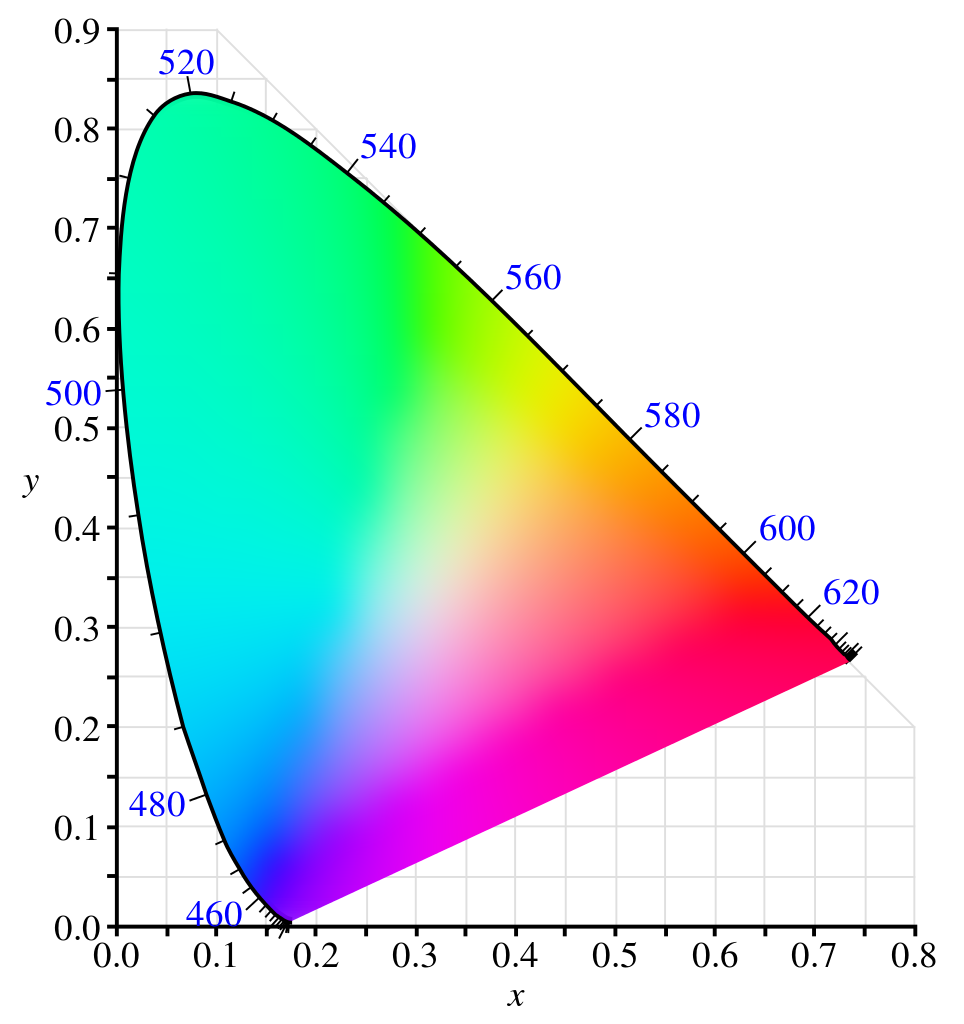
\includegraphics[width=.5\textwidth]{cie-cromaticity-diagram}
  % fonte https://en.wikipedia.org/wiki/File:CIE1931xy_blank.svg
  \caption[Diagrama de cromaticidade CIE 1931]{Diagrama de cromaticidade CIE 1931. Os pontos que representam as cores puras no espectro eletromagnético são rotulados de acordo com os seus comprimentos de onda e estão localizados ao longo da curva que vai da extremidade direita do eixo $x$, correspondente à cor vermelha, até a extremidade esquerda do mesmo eixo, correspondente à cor violeta, formando um polígono parecido com uma ferradura. Os pontos internos correspondem a todas as combinações possíveis de cores visíveis. Fonte: \citet{ben:09}.}
  \label{fig:cie-cromaticity-diagram} 
\end{figure}

As coordenadas $(x = 1/3, y = 1/3)$ correspondem à localização da luz branca, também conhecida como ponto branco, e servem de referência no processo de captura de imagem, codificação ou reprodução.

O CIE também derivou e padronizou outros dois modelos de cores a partir da especificação do CIE XYZ e, da mesma maneira, são independente de dispositivo. Ambos são perceptualmente uniformes, ou seja, distâncias perceptuais iguais separam todas as cores \citep{vezhnevets:03}. Como exemplo, a escala de cinzas do espaço deve permitir uma transição suave entre o preto e o branco.

O primeiro deles foi concebido para reduzir o problema de não uniformidade perceptual. Alguns diagramas de Escala Uniforme de Cromaticidade (UCS) foram propostos com base em equações matemáticas para transformar os valores XYZ ou as coordenadas $x, y$ em um novo conjunto de valores $(u, v)$, o que deu origem ao diagrama de cromaticidade 1960 CIE $uv$ \citep{gevers:12}.

Ainda com resultados insatisfatórios, o CIE fez uma nova mudança multiplicando o componente $v$ por um fator 1,5. Além disso, a escala de luminosidade dada pelo componente Y foi substituída por $L^* = [0, 100]$ para melhor representar as diferenças na luminosidade que são equivalentes. Esta revisão originou o modelo de cores \textbf{CIE 1976 $L^*u^*v^*$}, comumente conhecido pela sigla CIELUV \citep{gevers:12}.

Em 1976 o CIE adotou um novo modelo de cores, baseado no modelo $L, a, b$, proposto por Richard Hunter em 1948, que melhor representava o espaçamento uniforme das cores. Denominado \textbf{1976 CIE $L^*a^*b^*$} e conhecido pela sigla CIELAB, é um espaço baseado em cores oponentes \footnote{Teoria iniciada por volta do ano de 1500 quando Leonardo da Vinci concluiu que as cores são produzidas pela mistura de amarelo e azul, verde e vermelho, e branco e preto. Em 1950 houve a confirmação desta teoria quando sinais de cores oponentes foram detectados na conexão óptica entre a retina e o cérebro \citep{gevers:12}.} no qual os estímulos de cor da retina são convertidos para distinções entre claro e escuro, vermelho e verde, e azul e amarelo, representados pelos eixos $L^*$, $a^*$, e $b^*$, respectivamente \citep{gevers:12}.

%% ------------------------------------------------------------------------- %%
\subsection{Modelo RGB}\index{cores!modelo RGB}
\label{sec:modelo_cores_rgb}

O modelo RGB, acrônimo do inglês \textit{Red, Green, Blue}, é um modelo de cores aditivo no qual as três cores primárias vermelho, verde e azul são somadas para produzir as demais \citep{gonzalez:02}.

Esse sistema foi baseado na teoria tricromática de Thomas Young e Hermann Helmholtz em meados do século 19 e pode ser representado graficamente
através do cubo unitário definido sobre os eixos R, G e B, como ilustrado na figura~\ref{fig:rgb-cube} \citep{konstantinos:00}.

\begin{figure}[!h]
  \centering
  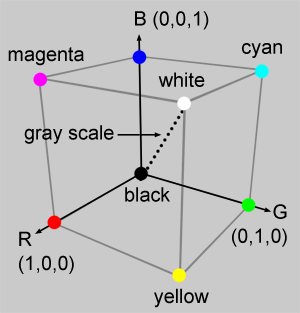
\includegraphics[width=.35\textwidth]{rgb-cube}
  % http://www.scratchapixel.com/old/lessons/3d-basic-lessons/lesson-5-colors-and-digital-images/color-spaces/
  \caption[Cubo unitário representando as cores do modelo RGB]{Cubo unitário representando as cores do modelo RGB. A origem, dada pelo vértice $(0, 0, 0)$, representa a cor preta. Já o vértice $(1, 1, 1)$, oposto à origem, representa a cor branca. Os vértices destacados sobre os eixos representam as cores primárias e os demais são o complemento de cada uma delas. Cada ponto no interior do cubo corresponde a uma cor que pode ser representada pela tripla $(r, g, b)$, onde $r, g, b \in [0, 1]$. Os tons de cinza são representados ao longo da diagonal principal do cubo, sendo que cada ponto ao longo dessa diagonal é formado por contribuições iguais de cada primária. Fonte: adaptado de \citet{gonzalez:02}.}
  \label{fig:rgb-cube} 
\end{figure}

Vale ressaltar que existem duas formas de representar o espaço RGB: linear e não linear. O sistema supra citado mostra o modelo não linear, cuja sigla é $R'G'B'$, e é o mais utilizado por dispositivos e aplicações pela sua similaridade com o sistema visual humano. Na literatura, esse sistema é frequentemente citado com a sigla RGB, o que torna a nomenclatura dúbia, uma vez que o modelo linear também é denominado RGB e, portanto, a conversão entre os espaços de cores deve ser feita com certa cautela. Também é importante citar que os valores RGB lineares são raramente utilizados para representar uma imagem já que são, perceptualmente, altamente não uniformes \citep{konstantinos:00}.


%% ------------------------------------------------------------------------- %%
\subsection{Modelo CMY}\index{cores!modelo CMY}
\label{sec:modelo_cores_cmy}

O modelo CMY é baseado nas cores primárias complementares Ciano, Magenta e Amarelo e, diferentemente do RGB, é um modelo de cores subtrativo no qual as cores são geradas subtraindo-se o comprimento da onda dominante da luz branca e, por isso, a cor resultante corresponde à luz que é refletida \citep{gonzalez:02}.

Uma maneira de obter o sistema CMY é:\\
\begin{equation}
  \begin{bmatrix}
    C \\ M \\ Y
  \end{bmatrix} = 
  \begin{bmatrix}
    B \\ R \\ R
  \end{bmatrix} +
  \begin{bmatrix}
    G \\ B \\ G
  \end{bmatrix}
\end{equation}

ou ainda, efetuando uma mudança de coordenadas subtraindo-se as cores primárias R, G e B da cor branca $W = (1, 1, 1)$ \citep{gonzalez:02}:
\begin{equation}
  \begin{bmatrix}
    C \\ M \\ Y
  \end{bmatrix} = 
  \begin{bmatrix}
    1 \\ 1 \\ 1
  \end{bmatrix} -
  \begin{bmatrix}
    R \\ G \\ B
  \end{bmatrix}
\end{equation}

Assim como o RGB, o CMY é dependente de dispositivo. O modelo é amplamente utilizado em equipamentos que depositam pigmentos coloridos sobre papel, tais como impressoras ou fotocopiadoras coloridas. A figura \ref{fig:cmy-model} mostra como os componentes do modelo são combinados para gerar as demais cores.

\begin{figure}[!h]
  \centering
  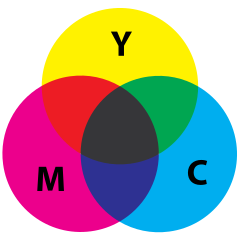
\includegraphics[width=.25\textwidth]{cmy-model}
  % https://en.wikipedia.org/wiki/File:SubtractiveColor.svg
  \caption[Modelo de cores subtrativo CMY]{Modelo de cores subtrativo CMY. É interessante observar que a intersecção de amarelo com magenta gera a cor vermelha, magenta com ciano gera a cor azul e ciano com amarelo gera a cor verde. Fonte: \citet{rus:08}.}
  \label{fig:cmy-model}
\end{figure}

A sobreposição das cores primárias CMY em iguais quantidades para gerar a cor preta tipicamente cria uma tonalidade próxima ao marrom ou verde escuro. Para evitar esse efeito indesejado, normalmente adiciona-se o componente de cor preta no sistema, representado pela letra K, obtendo-se um novo modelo conhecido como \textbf{CMYK} \citep{gonzalez:02}.

%% ------------------------------------------------------------------------- %%
\subsection{Modelo de cores da família YUV}\index{cores!modelos da família YUV}
\label{sec:modelo_cores_yuv}

O termo YUV refere-se a uma família de espaços de cores dos quais a informação de luminância, representada pelo componente Y, é codificada separadamente da crominância, dada pelos componentes U e V. Os componentes U e V são representações dos sinais da diferença do azul subtraído da luminância (B-Y) e vermelho subtraído da luminância (R-Y). É utilizado para representar as cores em sistemas de transmissão analógica de televisão nos padrões Linha de Fase Alternada (PAL) e Cor Sequencial Com Memória (SECAM) \citep{pedrini:08}.

A tranformação do espaço RGB para YUV é dada por:\\
\begin{equation}
  \begin{bmatrix}
    Y \\ U \\ V
  \end{bmatrix} = 
  \begin{bmatrix}
     0.299 &  0.587 &  0.114 \\
    -0.147 & -0.289 &  0.436 \\
     0.615 & -0.515 & -0.100 \\
  \end{bmatrix}
  \begin{bmatrix}
    R \\ G \\ B
  \end{bmatrix}
\end{equation}
onde $0 \leq R, G, B \leq 1$.

Análogo ao YUV, o modelo \textbf{YIQ} foi adotado em 1950 pelo Comitê Nacional do Sistema de Televisão (NTSC), um padrão americano para transmissão de sinal de televisão a cores. Nesse modelo, o componente Y corresponde à luminância e os componentes I (matiz) e Q (saturação) codificam a informação de crominância \citep{pedrini:08}.

A tranformação do espaço RGB para YIQ é dada por:\\
\begin{equation}
  \begin{bmatrix}
    Y \\ I \\ Q
  \end{bmatrix} = 
  \begin{bmatrix}
    0.299  &  0.587 &  0.114 \\
    0.596  & -0.275 & -0.321 \\
    0.212  & -0.523 & -0.311 \\
  \end{bmatrix}
  \begin{bmatrix}
    R \\ G \\ B
  \end{bmatrix}
\end{equation}
onde $0 \leq R, G, B \leq 1$.

Um outro modelo de cores da família YUV é o \textbf{YCbCr}, definido matematicamente por uma transformação de coordenadas em relação a algum espaço RGB \citep{pedrini:08}.

O modelo YCbCr é largamente utilizado em vídeos digitais. Nesse modelo, o componente Y representa a luminância, o componente Cb dá a medida da diferença entre a cor azul e um valor de referência, análogo ao componente Cr que é a medida da diferença entre a cor vermelha e um valor de referência \citep{pedrini:08}.

A conversão do espaço RGB para YCbCr é dada por:\\
\begin{equation}
  \begin{bmatrix}
    Y \\ Cb \\ Cr
  \end{bmatrix} = 
  \begin{bmatrix}
     0.299 &  0.587 &  0.114 \\
    -0.169 & -0.331 &  0.5   \\
     0.5   & -0.419 & -0.081 \\
  \end{bmatrix}
  \begin{bmatrix}
    R \\ G \\ B
  \end{bmatrix}
\end{equation}


%% ------------------------------------------------------------------------- %%
\subsection{Modelo de cores da família HSI}\index{cores!modelos da família HSI}
\label{sec:modelo_cores_hsi}

Modelos baseados no Matiz, Saturação e Intensidade (HSI) são mais adequados para aplicações de processamento de imagens, do ponto de vista do usuário, pela correlação com a percepção humana da cor \citep{konstantinos:00}.

Nesse modelo, assim como no YIQ, a intensidade dada pelo componente I é decomposta da informação de crominância, representada pelo matiz (H) e saturação (S) \citep{konstantinos:00}. A combinação desses componentes resulta em uma estrutura piramidal que pode ser vista na figura~\ref{fig:hsi-model}.

\begin{figure}[!h]
  \centering
  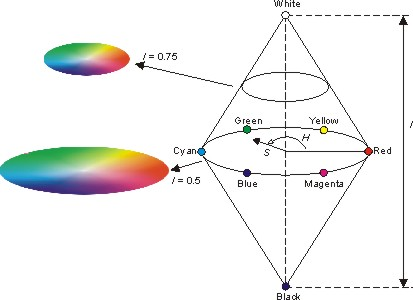
\includegraphics[width=.6\textwidth]{hsi-model}
  % http://www.blackice.com/images/HSIColorModel.jpg
  \caption[Representação gráfica do modelo HSI]{Representação gráfica do modelo HSI. O matiz descreve a cor em si, sob a forma de um ângulo $\theta$, onde $\theta \in [0, 360]$. O vermelho está situado a 0 grau, amarelo a 60, verde a 120 e assim sucessivamente. O componente de saturação, que varia entre 0 e 1, indica o quanto a cor está poluída com a cor branca. A escala de intensidade está entre $[0, 1]$, onde 0 significa preto e 1, branco.}
  \label{fig:hsi-model} 
\end{figure}

A transformação dos componentes do espaço RGB para HSI é dada pelas equações:
\begin{align}
\label{eq:rgb_para_hsi}
\begin{split}
  \theta &= cos^{-1} \bigg( \frac{(R - G) + (R - B)}{2 \sqrt{(R - G)^2 + (R - B)(G - B)}} \bigg)
  \\[0.5em]
  H &= \begin{cases}
            \theta,       & \text{se}\ B \leq G\\
            360 - \theta, & \text{caso contrário}\\
       \end{cases}
  \\[0.5em]
  S &= 1 - \frac{3 min(R, G, B)}{R + G + B}
  \\[0.5em]
  I &= \frac{R + G + B}{3}
\end{split}
\end{align}

É importante ressaltar que os valores R, G e B devem estar normalizados no intervalo entre 0 e 1. A intensidade $I$ e a saturação $S$ também estão normalizadas entre 0 e 1.

Outro modelo desta família é formado pelos componentes Matiz, Saturação e Luminância (\textbf{HSV}) e sua representação gráfica tridimensional é uma pirâmide hexagonal derivada do cubo RGB \citep{pedrini:08}.

Os vários matizes estão representados na parte superior da pirâmide, a saturação é medida ao longo do eixo horizontal e a luminância é medida ao longo do eixo vertical, que passa pelo centro da pirâmide. O matiz, que corresponde às arestas ao redor do eixo vertical, varia de 0 (vermelho) a 360 graus e o ângulo entre os vértices é de 60 graus. A saturação varia de 0 a 1 e é representada como sendo a razão entre a pureza de um determinado matiz e a sua pureza máxima, ou seja, quando $S = 1$. A luminância varia de 0, no pico da pirâmide representando a cor preta, a 1 na base, onde as intensidades das cores são máximas \citep{pedrini:08}.

A conversão do espaço RGB para HSV é dada pelas equações:
\begin{align}
\label{eq:rgb_para_hsv}
\begin{split}
  H &=  \begin{cases}
            60\ffrac{(G - B)}{M - m}, & \text{se}\ M = R\\[0.7em]
            60\ffrac{(B - R)}{M - m} + 120, & \text{se}\ M = G\\[0.7em]
            60\ffrac{(R - G)}{M - m} + 240, & \text{se}\ M = B
       \end{cases}
  \\[0.5em]
  S &=  \begin{cases}
            \ffrac{(M - m)}{M}, \quad &\text{se}\ M \neq 0\\[0.7em]
            0, \quad &\text{caso contrário}\\
       \end{cases}
  \\[0.5em]
  V &= M
\end{split}
\end{align}

\noindent onde $m = min(R, G ,B)$ e $M = max(R, G ,B)$. A luminância $V$ e a saturação $S$ estão normalizadas entre 0 e 1. Já o matiz $H$ varia entre 0 e 360 graus.

Da mesma forma que o HSV, o modelo Matiz, Saturação e Luminosidade (\textbf{HSL}) é uma representação tridimensional e é formado por dois cones de altura 1, cujas bases são coincidentes \citep{pedrini:08}.

O matiz é determinado pelos pontos no círculo das bases comuns aos cones. A saturação varia de 0 a 1, conforme a distância ao eixo do cone. A luminosidade está ao longo do eixo vertical comum aos dois cones e varia na escala $[0, 1]$, onde 0 significa preto e 1, branco \citep{pedrini:08}.

A conversão do espaço RGB para HSL é dada pelas equações:
\begin{align}
\label{eq:rgb_para_hsl}
\begin{split}
  H &=  \begin{cases}
            60\ffrac{(G - B)}{M - m}, & \text{se}\ M = R\\[0.7em]
            60\ffrac{(B - R)}{M - m} + 120, & \text{se}\ M = G\\[0.7em]
            60\ffrac{(R - G)}{M - m} + 240, & \text{se}\ M = B
       \end{cases}
  \\[0.5em]
  S &=  \begin{cases}
            \ffrac{(M - m)}{M + m}, & \text{se}\ 0 < L \leq 0,5\\[0.7em]
            \ffrac{(M - m)}{2 - (M + m)}, & \text{se}\ L > 0,5\\[0.5em]
            0, & \text{se}\ M = m\\
       \end{cases}
  \\[0.5em]
  L &= \frac{M + m}{2}
\end{split}
\end{align}

\noindent onde $m = min(R, G ,B)$ e $M = max(R, G ,B)$. A luminância $V$ e a saturação $S$ estão normalizadas entre 0 e 1. Observe que a transformação do matiz $H$ é a mesma utilizada na conversão do espaço RGB para HSV em \ref{eq:rgb_para_hsv} e varia entre 0 e 360 graus.

Todos os modelos de cores desta família têm a propriedade de se pensar em cores mais claras, obtidas pelo aumento do brilho ou luminosidade, e mais escuras, pela diminuição dos mesmos valores. As cores intermediárias são produzidas pela diminuição da saturação \citep{pedrini:08}.

%% ------------------------------------------------------------------------- %%
\section{Teoria \emph{fuzzy}}\index{fuzzy!teoria}
\label{sec:teoria_fuzzy}

Em muitos problemas, não há dificuldade em determinar se um dado elemento é ou não parte de um grupo. Essa ideia vem da teoria clássica de conjuntos e é embasada no conceito fundamental de conjunto \citep{chen:00}. Pode-se, por exemplo, afirmar que o número $7$ pertence ao conjunto dos números naturais e, da mesma maneira, que o número $-7$ não pertence a esse mesmo conjunto. Este é um caso clássico em que a aplicação da lógica booleana é bem sucedida. Em outras palavras, quando questionado se o número $7$ pertence ao conjunto dos naturais tem-se, apenas, duas respostas possíveis: sim ou não.

Entretanto, há inúmeros indivíduos ou observações na natureza que nem sempre podem ser classificados de tal forma, pelo fato de que a relação de pertinência não é bem definida \citep{pedrycz:98}. Como exemplo, o conjunto das pessoas altas, os números reais aproximadamente zero ou o grupo de alunos mais inteligentes da escola. Ocorre que, nesses casos, a aplicação da lógica booleana para classificar elementos como parte de um grupo ou não é imprecisa. Em outras palavras, se tomado $x = 1,70m$ como o limiar que separa as pessoas altas das baixas, fica evidente que a utilização da lógica booleana não resulta em interpretações realísticas, pois uma pessoa com $1,69m$ é, portanto, baixa ou, pode-se dizer ainda, que não pertence ao grupo das pessoas altas. Ora, apenas $1$ centímetro separa tal pessoa de um grupo ou de outro. Analogamente, uma pessoa com $1,71m$ está muito próxima de pertencer ao grupo das pessoas baixas.

Claramente, a resposta a ser obtida quando da análise de possibilidades desse tipo é fortemente dependente do contexto, pois há um alto grau de incerteza inerente aos elementos e conjuntos sendo considerados.

O conceito de incerteza mudou gradativamente na ciência e na matemática. Na ciência, esta mudança foi manifestada por uma transição gradual da visão tradicional, que insiste que a incerteza é indesejável e, por esta razão, ela deve ser evitada por todos os meios possíveis, para uma visão alternativa, que é tolerante à incerteza. De acordo com a visão tradicional, a ciência deve esforçar-se de certeza em todas as suas manifestações, ou seja, com precisão, especificidade, nitidez, consistência e, por conseguinte, a incerteza é considerada como não científica. De acordo com a visão alternativa, a dúvida é considerada essencial para a ciência; não é só uma praga inevitável, mas tem, de fato, uma grande utilidade \citep{klir:95}.

E com base na ideia moderna de que a incerteza é algo útil na ciência é que Zadeh convergiu para um de seus mais importantes trabalhos: a teoria de conjuntos \emph{fuzzy}, cuja abordagem sobre conjuntos dá-se sob a ótica de que os limites entre eles não são precisos e, portanto, é possível estabelecer funções que forneçam um certo grau de pertinência\index{pertinência!grau de} de um elemento a um dado conjunto \citep{zadeh:65}.

A capacidade de conjuntos \emph{fuzzy} expressarem transições graduais de pertinência e não pertinência tem uma grande utilidade. Ela fornece não só uma representação significativa e poderosa da medida de incerteza, mas também uma forma de expressar conceitos vagos em linguagem natural \citep{klir:95}. Voltando ao exemplo do conjunto de pessoas altas, em vez de descrever a altura de uma pessoa com exatidão em metros ou centímetros, pode-se apenas dizer que ela é alta, baixa ou mediana. Cada um desses conjuntos pode ser um conjunto \emph{fuzzy}, onde um valor 1 é atribuído a um membro que está totalmente incluído em um deles, ou 0 caso contrário. Valores intermediários nessa escala indicam que o elemento está parcialmente em um dos conjuntos.

A seção \ref{sec:conjuntos_fuzzy} explicita algumas das definições formais e conceitos básicos da teoria dos conjuntos \emph{fuzzy} proposta por Zadeh.

%% ------------------------------------------------------------------------- %%
\subsection{Conjuntos \emph{fuzzy}}\index{fuzzy!conjuntos}
\label{sec:conjuntos_fuzzy}
A teoria de conjuntos clássicos está baseada em uma função, geralmente conhecida como função característica, dada por:

\begin{equation}
  \mu_A(x) =  \begin{cases}
                1 \quad \text{se}\ x \in A \\
                0 \quad \text{se}\ x \notin A
              \end{cases}
\end{equation}
onde $U$ é o conjunto Universo, $A$ é um subconjunto de $U$ e $x$ é um elemento de $U$ \citep{klir:95}.

Portanto, a função característica é um mapeamento dos elementos de $U$ no conjunto binário $\{0, 1\}$, formalmente definida como:

\begin{equation}
  \mu_A =  U \rightarrow \{0, 1\}
\end{equation}

Sendo assim, a função característica determina que, de acordo com algum critério, $\forall x \in U$, se $\mu_A(x) = 1$, então $x$ é um membro de $A$, por outro lado, quando $\mu_A(x) = 0$, $x$ não é um membro de $A$.

Quanto aos conjuntos \emph{fuzzy}, basta generalizar a função característica aplicada nos conjuntos clássicos no intervalo $[0, 1]$ para obter-se um conjunto "fuzzificado", ou seja, o grau de pertinência de um elemento $x$ passa, agora, a ser expresso em termos contínuos. Em outras palavras, o elemento $x$ pertence ao subconjunto $A$ de $U$ com algum grau de pertinência obtido do intervalo $[0, 1]$. Formalmente, tem-se:

\begin{equation}
  \mu_A =  U \rightarrow [0, 1]
\end{equation}

Cabe aqui citar a definição de conjuntos \emph{fuzzy} dada por Zadeh que designa um conjunto \emph{fuzzy} como uma classe de objetos com um grau de pertinência contínuo. Tal conjunto é caracterizado por uma função de pertinência (característica), que atribui a cada objeto um grau de pertinência que varia entre zero e um. As noções de inclusão, união, intersecção, complemento, relação, convexidade, etc., oriundas da teoria de conjuntos clássica, são estendidas a esses conjuntos \citep{zadeh:65}.

% definição de conjunto fuzzy
\begin{defn}
Um conjunto \emph{fuzzy} $A$ é um subconjunto do conjunto universo $U$ formado por pares ordenados de um elemento qualquer $x$ e seu grau de pertinência dado por $\mu_A(x)$, da forma:

\begin{equation}
  A =  \{(x, \mu_A(x)) \ |\ x \in U\}
\end{equation}
\end{defn}

O universo de discurso $U$ pode ser composto por elementos discretos ou ser um espaço contínuo. A mesma implicação vale para o subconjunto $A$. No caso em que $U$ é um conjunto discreto e finito, tal que $U = \{x_1, x_2, x_3, \ldots, x_n\}$, pode-se simplesmente enumerar os seus elementos, juntamente com seus graus de pertinência, como segue:

\begin{equation}
  A =  \frac{\mu_A(x_1)}{x_1} + \frac{\mu_A(x_2)}{x_2} + \ldots + \frac{\mu_A(x_n)}{x_n} = \sum_{i=1}^n \frac{\mu_A(x_i)}{x_i}
\label{equ:conjunto_fuzzy_finito}
\end{equation}

É importante ressaltar que o somatório em \ref{equ:conjunto_fuzzy_finito} não significa uma adição algébrica, mas sim a união de todos os pares ordenados de $x$ e $\mu_A(x)$ que formam o conjunto $A$ \citep{klir:95}.

\begin{exmp}
\textcolor{red}{Colocar um exemplo aqui de conjunto fuzzy que tenha sentido com o restante do texto, posteriormente. Pode ser pessoas altas, para ligar com o exemplo supra citado.}
\end{exmp}

% definição de altura
\begin{defn}
A altura de $A$, denotado por $altura(A)$, corresponde ao limite superior do codomínio da sua função de pertinência, da forma:

\begin{equation}
  altura(A) = \{\mu_A(x) \ |\ x \in U\}
\label{equ:conjunto_fuzzy_altura}
\end{equation}

\end{defn}

% definição de conjunto normalizado
\begin{defn}
Um conjunto \emph{fuzzy} $A$ é dito normalizado se existe pelo menos um elemento $x \in U$, tal que $\mu_A(x) = 1$.
\label{def:conjunto_fuzzy_normalizado}
\end{defn}

A definição de conjunto \emph{fuzzy} normalizado implica que pelo menos um membro de $A$ alcança o grau de pertinência máximo possível. Note que a definição em \ref{def:conjunto_fuzzy_normalizado} considera que os valores dos graus de pertinência variam no intervalo fechado entre 0 e 1. Logo, no mínimo um elemento deve ter um grau de pertinência 1 para que $A$ possa ser considerado, de fato, normalizado. Observe que, decorrente dessa afirmação, imediatamente tem-se que $altura(A) = 1$.

% definição de suporte
\begin{defn}
O suporte de um conjunto \emph{fuzzy} $A$ em $U$, denotado por $suporte(A)$, é o conjunto dado por:

\begin{equation}
  suporte(A) = \{x \in U \ |\ \mu_A(x) > 0 \}
\label{equ:conjunto_fuzzy_suporte}
\end{equation}

\end{defn}

Em outras palavras, o conjunto suporte é um conjunto clássico ou conjunto ordinário que contém todos os elementos de $U$ cujo grau de pertinência é maior do que zero em $A$. Denomina-se por conjunto unitário ou \emph{singleton} um conjunto \emph{fuzzy} cujo suporte é um único ponto, por exemplo $w$, tal que $\mu_A(w) = 1$.

% definição de alfa corte
\begin{defn}
Um $\alpha$\emph{-corte}, também conhecido por $\alpha$\emph{-nível}, é o subconjunto clássico de elementos cujo grau de pertinência é maior ou igual a um valor $\alpha$, formalmente:

\begin{equation}
  \alpha\emph{-corte(A)} = \{x \in U \ |\ \mu_A(x) \geq \alpha \}
\label{equ:conjunto_fuzzy_alpha_corte}
\end{equation}
\end{defn}

% definição de núcleo
\begin{defn}
O núcleo ou \emph{kernel} de um conjunto \emph{fuzzy} $A$ em $U$, é o conjunto de elementos pertencentes inteiramente à $A$, da forma:

\begin{equation}
  \emph{núcleo}(A) = \{x \in U \ |\ \mu_A(x) = 1 \}
\label{equ:conjunto_fuzzy_kernel}
\end{equation}
\end{defn}

Vale destacar que, por construção, o núcleo do conjunto $A$ está contido no conjunto suporte, o que pode ser representado formalmente como $\emph{núcleo}(A) \subseteq suporte(A)$.

A figura~\ref{fig:fuzzy_definitions} mostra graficamente algumas das propriedades definidas acima.

\begin{figure}[!h]
  \centering
  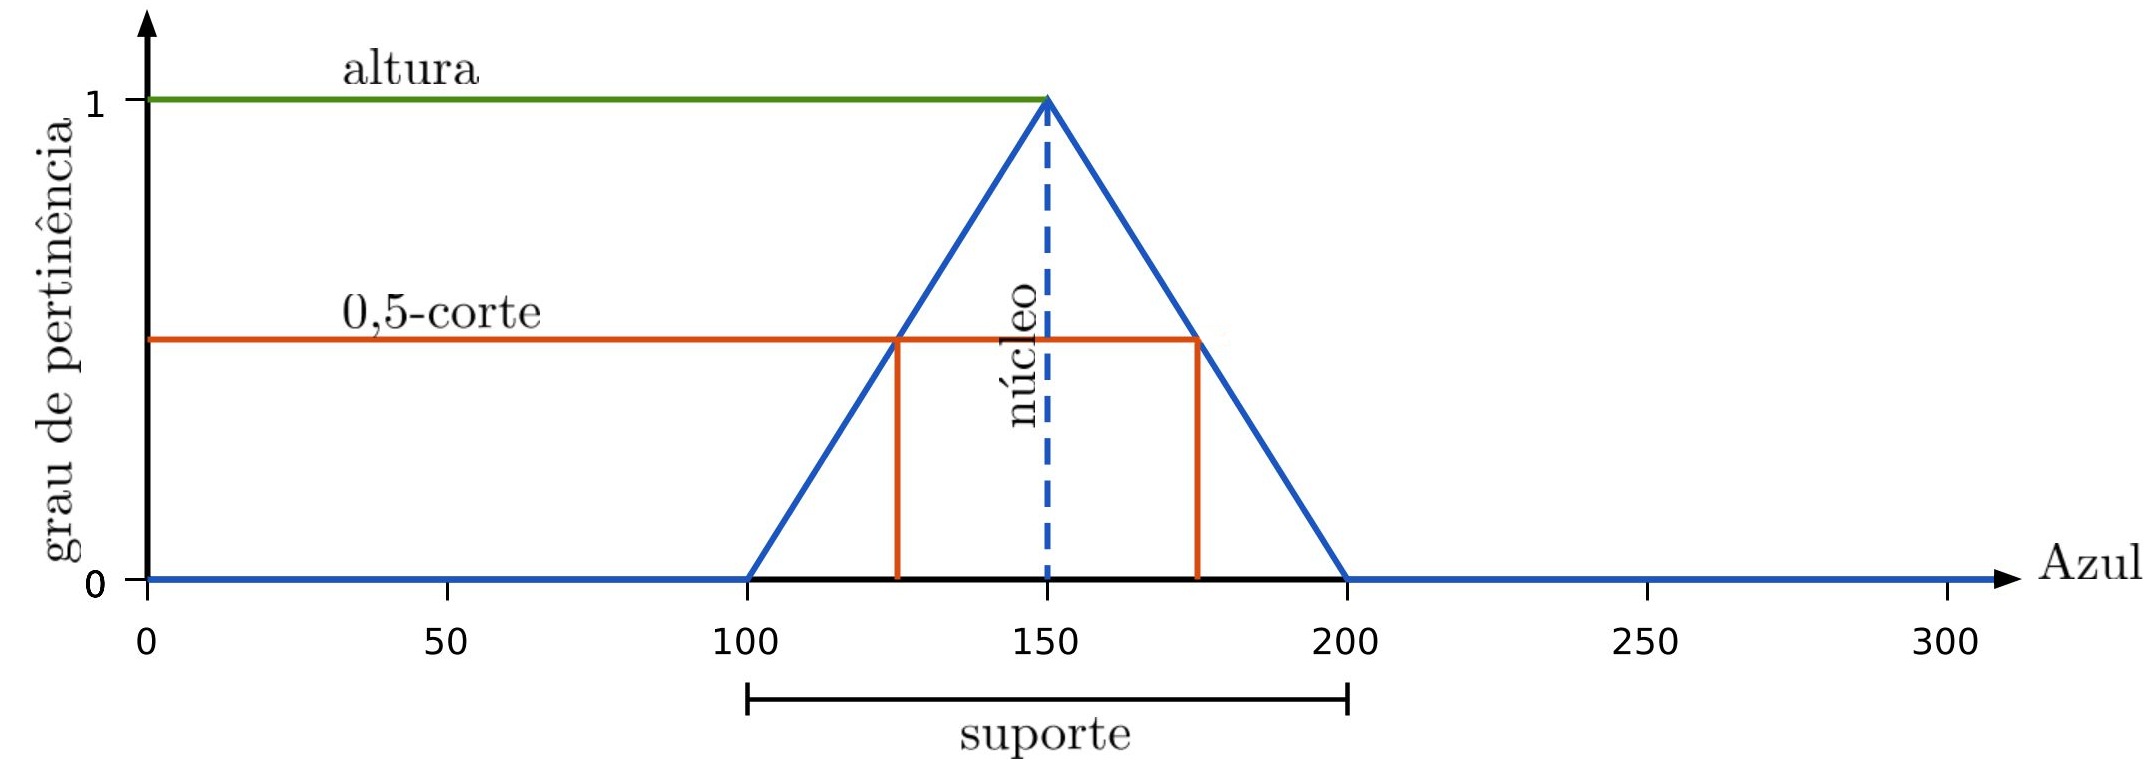
\includegraphics[width=1\textwidth]{fuzzy_definitions}
  % source MIT class notes
  \caption{Representação gráfica das principais propriedades dos conjuntos fuzzy. \textcolor{red}{Detalhar melhor e corrigir a imagem.}}
  \label{fig:fuzzy_definitions} 
\end{figure}

%% ------------------------------------------------------------------------- %%
\subsection{Operações entre conjuntos \emph{fuzzy}}\index{fuzzy!operações entre conjuntos}
\label{sec:operacoes_conjuntos_fuzzy}

Assim como na teoria de conjuntos clássica, há basicamente três operações que podem ser estendidas aos conjuntos \emph{fuzzy}. Essas operações são a união, a intersecção e o complemento, sendo representadas pelos operadores lógicos de conjunção (\textbf{OU}), disjunção (\textbf{E}) e complemento (\textbf{NÃO}), respectivamente. As operações básicas formam o que é conhecido como operações padrão em conjuntos \emph{fuzzy} \citep{klir:95}.

Tais operações são realizadas sobre suas respectivas funções de pertinência e há muitas formalizações matemáticas possíveis para os operadores que representam-nas. O par de operadores mais amplamente utilizado é o operador de mínimo ($min$) e máximo ($max$), que são semelhantes aos operadores produto e soma da álgebra elementar e utilizados para expressar a conjunção e disjunção, respectivamente \citep{thole:79}.

Seja dois conjuntos \emph{fuzzy} $A$ e $B$, definidos sobre um mesmo universo de discurso $U$. Utilizando as funções $max$ e $min$, tem-se que \citep{klir:95}:

% definição de união
\begin{defn}
\label{def:conjunto_fuzzy_uniao}
O conjunto união é formado por todos os valores máximos entre dois conjuntos \emph{fuzzy} $A$ e $B$, onde $A, B \in U$, da forma:

\begin{equation}
  \mu_A(x) \cup \mu_B(x) = max\{\mu_A(x), \mu_B(x)\}, \quad \forall x \in U
\end{equation}
\end{defn}

A figura~\ref{fig:fuzzy_operacoes_uniao} exibe graficamente dois conjuntos \emph{fuzzy} $A$ e $B$ quaisquer, bem como a área pertinente à união entre eles.

\begin{figure}[!h]
  \centering
  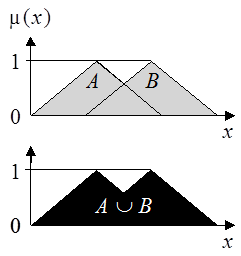
\includegraphics[width=.28\textwidth]{fuzzy_operacoes_uniao}
  \caption[Operação de união entre dois conjuntos fuzzy]{Representação gráfica da operação de união entre dois conjuntos fuzzy. A parte superior em cinza claro mostra os dois conjuntos fuzzy $A$ e $B$ em sobreposição. A união é destacada em preto na parte inferior. Adaptado de \citet{vrusias:06}.}
  \label{fig:fuzzy_operacoes_uniao}
\end{figure}

% definição de intersecção
\begin{defn}
\label{def:conjunto_fuzzy_interseccao}
O conjunto intersecção é formado por todos os valores mínimos entre dois conjuntos \emph{fuzzy} $A$ e $B$, onde $A, B \in U$, da forma:

\begin{equation}
  \mu_A(x) \cap \mu_B(x) = min\{\mu_A(x), \mu_B(x)\}, \quad \forall x \in U
\end{equation}
\end{defn}

A figura~\ref{fig:fuzzy_operacoes_interseccao} exibe graficamente dois conjuntos \emph{fuzzy} $A$ e $B$ quaisquer, bem como a área pertinente à intersecção.

\begin{figure}[!h]
  \centering
  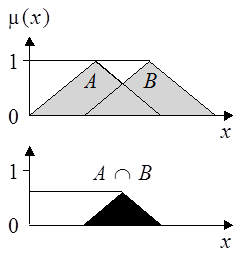
\includegraphics[width=.28\textwidth]{fuzzy_operacoes_interseccao}
  \caption[Operação de intersecção entre dois conjuntos fuzzy]{Representação gráfica da operação de intersecção entre dois conjuntos fuzzy. A parte superior em cinza claro mostra os dois conjuntos fuzzy $A$ e $B$ em sobreposição. A intersecção é destacada em preto na parte inferior. Adaptado de \citet{vrusias:06}.}
  \label{fig:fuzzy_operacoes_interseccao}
\end{figure}

% definição de complemento
\begin{defn}
\label{def:conjunto_fuzzy_complemento}
O complemento de um conjunto \emph{fuzzy} $A$, denotado por $\mu_{\bar{A}}(x)$, onde $A \in U$, é formado pela subtração entre o valor unitário e $\mu_A(x)$, da forma:

\begin{equation}
  \mu_{\bar{A}}(x) = 1 - \mu_A(x), \quad \forall x \in U
\end{equation}
\end{defn}

A figura~\ref{fig:fuzzy_operacoes_complemento} exibe graficamente um conjunto \emph{fuzzy} $A$ qualquer, bem como seu complemento.

\begin{figure}[!h]
  \centering
  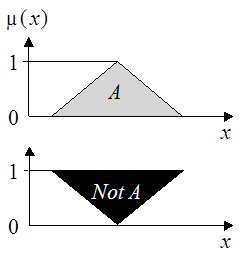
\includegraphics[width=.28\textwidth]{fuzzy_operacoes_complemento}
  \caption[Conjunto fuzzy e seu complemento]{Representação gráfica de um conjunto fuzzy e seu complemento. A parte superior em cinza claro mostra o conjunto fuzzy $A$. Seu complemento é destacado em preto na parte inferior. Adaptado de \citet{vrusias:06}.}
  \label{fig:fuzzy_operacoes_complemento}
\end{figure}

Além desses operadores, existem outros que podem ser utilizados para efetuar as operações lógicas. Um deles é a norma triangular, também denominada \textbf{\emph{norma-t}}. Outro é a co-norma triangular, usualmente denominada por \textbf{\emph{co-norma-t}} ou \textbf{\emph{norma-s}}. Os operadores utilizados para a intersecção de conjuntos \emph{fuzzy} pertencem à classe \emph{norma-t}. Os operadores utilizados para a união de conjuntos \emph{fuzzy} pertencem à classe \emph{co-norma-t} ou \emph{norma-s} \citep{zimmermann:01}.

Ambas \emph{norma-t} e \emph{norma-s} são funções binárias do tipo $[0, 1] \times [0, 1] \rightarrow [0, 1]$, que devem satisfazer algumas propriedades, tais como, monotonicidade, comutatividade, associatividade e condições de contorno \footnote{As propriedades não serão expressas neste trabalho, embora sejam amplamente conhecidas, exceto pelas condições de contorno. Mais detalhes podem ser vistos em \citet{zimmermann:01}.}. Os operadores $max$ e $min$ satisfazem tais propriedades e, por essa razão, podem ser utilizados nas operações lógicas \emph{fuzzy} \citep{zimmermann:01}.


%% ------------------------------------------------------------------------- %%
\subsection{Números \emph{fuzzy}}
\label{sec:numeros_fuzzy}
Conjuntos \emph{fuzzy} são composições de números \emph{fuzzy}, definidos em um universo discreto ou contínuo, de forma tal que a incerteza ou imprecisão associada a uma dada informação possa ser quantificada. Portanto, grandezas do tipo \emph{em torno de} 7, \emph{aproximadamente} -7, \emph{mais ou menos} 30 podem ser mapeadas e, consequentemente, interpretadas por números \emph{fuzzy}. Dessa forma, a concepção intuitiva sobre números aproximados ou intervalos pode ser capturada \citep{klir:95}.

\citet{klir:95} caracterizam um número \emph{fuzzy} como um tipo especial de conjunto \emph{fuzzy} definido no conjunto $\mathbb{R}$ dos números reais, cuja função de pertinência\index{pertinência!função de} tem a forma:
\begin{equation}
\label{eq:fuzzy_numero_reais}
  A = \mathbb{R} \rightarrow [0, 1]
\end{equation}

Para que $A$ seja, de fato, um número \emph{fuzzy}, o conjunto universo no qual $\mu_A$ está definida deve ser $\mathbb{R}$ e as seguintes propriedades devem ser satisfeitas \citep{barros:06}:
\begin{enumerate}[label=(\roman*)]
\item todos os $\alpha$\emph{-corte} de $A$ são não vazios, com $0 \leq \alpha \leq 1$;
\item todos os $\alpha$\emph{-corte} são intervalos fechados de $\mathbb{R}$;
\item $suporte(A) = \{x \in U \ |\ \mu_A(x) > 0\}$.
\end{enumerate}

De modo geral, números \emph{fuzzy} podem ser representados por funções parametrizadas. Algumas dessas funções serão apresentadas na seção \ref{sec:funcoes_pertinencia}.

%% ------------------------------------------------------------------------- %%
\subsection{Funções de pertinência}\index{pertinência!tipos de funções de}
\label{sec:funcoes_pertinencia}
As funções de pertinência são responsáveis por um aspecto fundamental na teoria de conjuntos \emph{fuzzy}. Como supra citado, elas permitem, por exemplo, que um número \emph{fuzzy} seja representado de forma paramétrica.

As funções lineares por partes são as mais populares devido à sua baixa complexidade e eficiência e, por conseguinte, baixo custo computacional necessário para o seu processamento, o que não ocorre com outros tipos de funções já que, em geral, não resultam em uma melhoria significativa na qualidade dos valores de saída dos sistemas \citep{yen:99}. Nesse contexto, as funções de pertinência mais comumente utilizadas são as \textbf{triangulares} e \textbf{trapezoidais}. Vale ressaltar que não é necessário que as funções sejam simétricas ou igualmente  espaçadas. Além disso, cada variável do problema pode ser modelada com funções de pertinência diferentes,  com  formas  e  distribuições  próprias, definidas  de  acordo com  as suas características e do contexto onde estão sendo aplicadas.

Em aplicações onde é necessário transições mais suaves, pode-se usar funções \textbf{gaussianas}, \textbf{sigmoidais}, dentre outras, desde que estejam definidas no intervalo [0, 1]. Algumas dessas funções serão apresentadas em \ref{def:funcao_fuzzy_triangular}, \ref{def:funcao_fuzzy_trapezoidal} e \ref{def:funcao_fuzzy_gaussiana}, com base nas definições de \citet{sumathi:10}.

% definição de função de pertinência triangular
\begin{defn}
\label{def:funcao_fuzzy_triangular}
Um número \emph{fuzzy} $A$ é dito triangular se sua função de pertinência, denotada por $\mu_{A}(x)$, é da forma:

\begin{equation}
  \mu_A(x) =  \begin{cases}
                \ffrac{x - a}{m - a}, & \text{se}\ a \leq x \leq m\\[0.5em]
                \ffrac{b - x}{b - m}, & \text{se}\ m \leq x \leq b\\[0.5em]
                0, & \text{caso contrário}
              \end{cases}
\end{equation}
\end{defn}
\noindent onde $m$ é o máximo grau de pertinência ou $altura(A)$, em geral $\mu_A(x) = 1$, e $a$ e $b$ os limites inferior e superior do intervalo, respectivamente, onde $\mu_A(x)$ é não nula.

A figura~\ref{fig:funcao_fuzzy_triangular} exibe o gráfico da função $\mu_A(x)$ de um número \emph{fuzzy} triangular $A$.

\begin{figure}[!h]
  \centering
  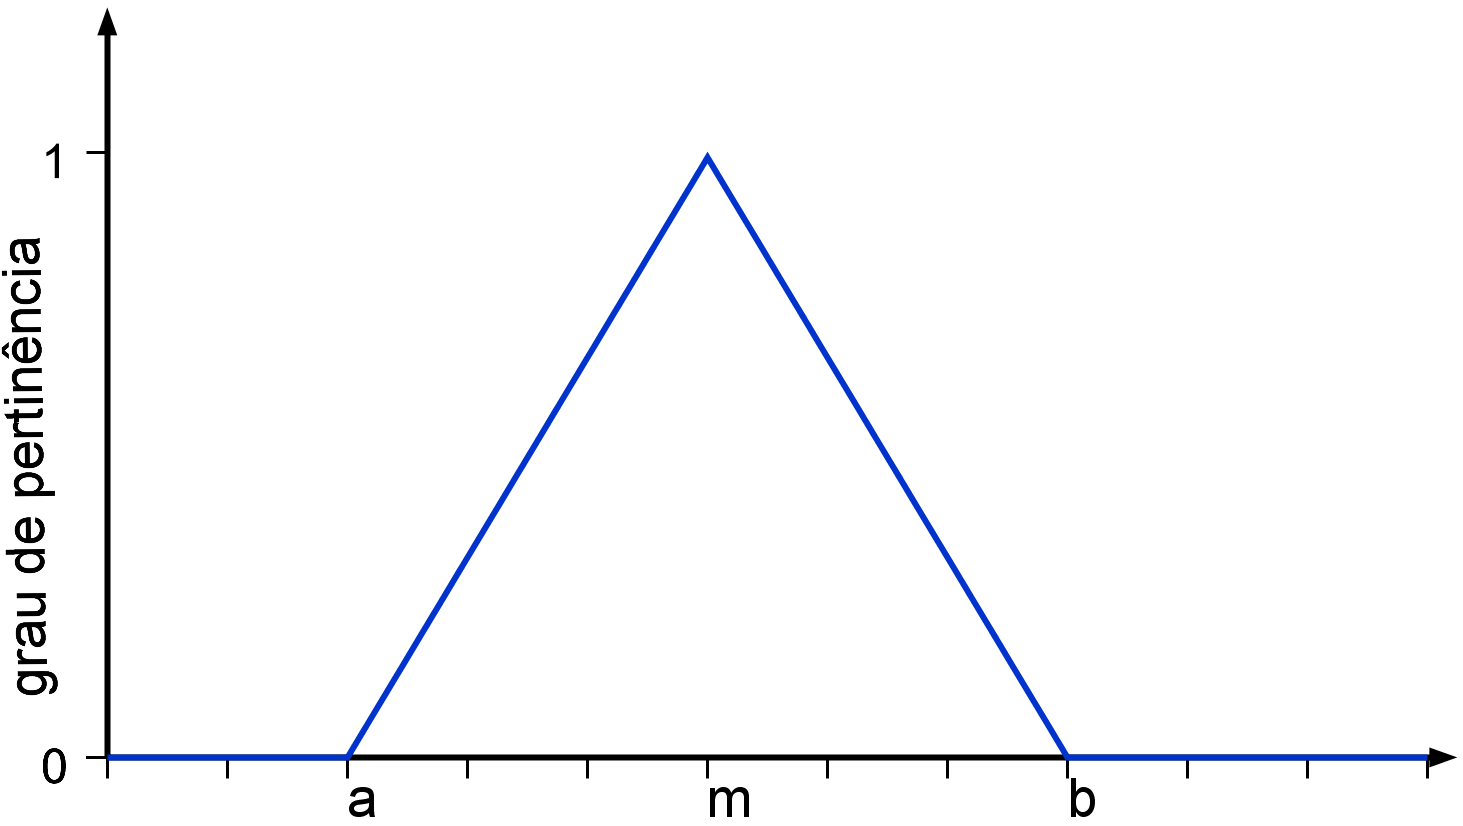
\includegraphics[width=.5\textwidth]{funcao_triangular}
  \caption[Gráfico da função de pertinência triangular]{Gráfico da função de pertinência triangular. Note que a forma é de um triângulo, que tem como base o intervalo $[a, b]$ e como $\emph{núcleo}(A)$ o vértice $(m, 1)$.}
  % http://www.dma.fi.upm.es/recursos/aplicaciones/logica_borrosa/web/fuzzy_inferencia/funpert_en.htm
  \label{fig:funcao_fuzzy_triangular}
\end{figure}

% definição de função de pertinência trapezoidal
\begin{defn}
\label{def:funcao_fuzzy_trapezoidal}
Um número \emph{fuzzy} $A$ é dito trapezoidal se sua função de pertinência, denotada por $\mu_{A}(x)$, é da forma:

\begin{equation}
  \mu_A(x) =  \begin{cases}
                \ffrac{x - a}{b - a}, & \text{se}\ a \leq x \leq b\\[0.5em]
                1, & \text{se}\ b \leq x \leq c\\[0.5em]
                \ffrac{d - x}{d - c}, & \text{se}\ c \leq x \leq d\\[0.5em]
                0, & \text{caso contrário}
              \end{cases}
\end{equation}
\end{defn}

A figura~\ref{fig:funcao_fuzzy_trapezoidal} exibe o gráfico da função $\mu_A(x)$ de um número \emph{fuzzy} trapezoidal $A$.

\begin{figure}[!h]
  \centering
  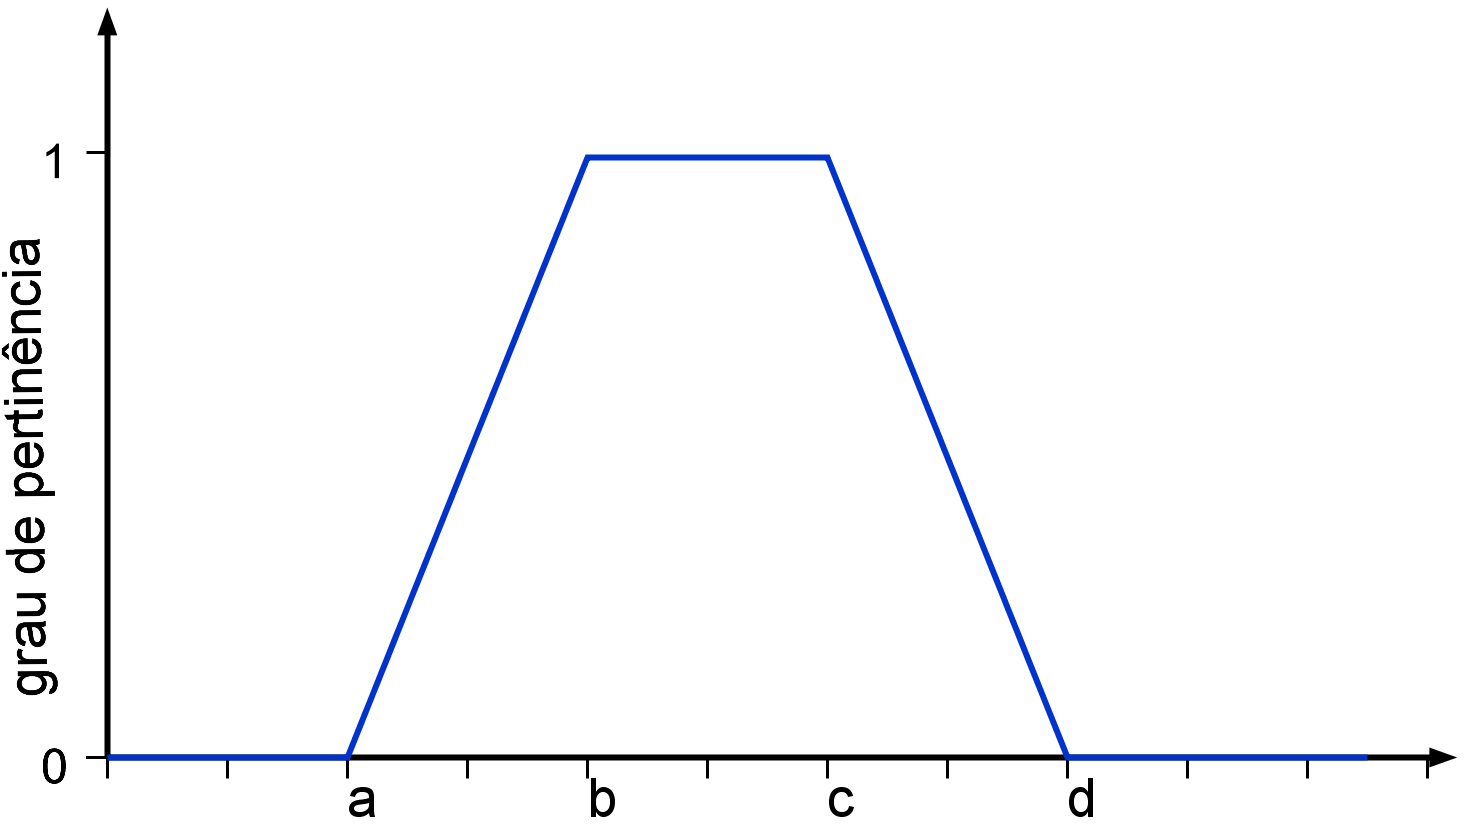
\includegraphics[width=.5\textwidth]{funcao_trapezoidal}
  \caption[Gráfico da função de pertinência trapezoidal]{Gráfico da função de pertinência trapezoidal. Aqui a forma é de um trapézio, sendo que $\mu_A(x)$ é nula para todo $x \notin [a, d]$, linearmente  crescente  até $altura(A)$, geralmente, para $x = b = c$, constante nesse valor para $x$ entre $b$ e $c$ e, finalmente, linearmente decrescente até zero em $x = d$.}
  % http://www.dma.fi.upm.es/recursos/aplicaciones/logica_borrosa/web/fuzzy_inferencia/funpert_en.htm
  \label{fig:funcao_fuzzy_trapezoidal}
\end{figure}

% definição de função de pertinência gaussiana
\begin{defn}
\label{def:funcao_fuzzy_gaussiana}
Um número \emph{fuzzy} $A$ é dito gaussiano se sua função de pertinência, denotada por $\mu_{A}(x)$, é da forma:

\begin{equation}
  \mu_A(x) =  \begin{cases}
                \exp{\big(-\ffrac{{(x - m)}^2}{\sigma} \big)}, & \text{se}\ m - \sigma \leq x \leq m + \sigma\\[0.5em]
                0, & \text{caso contrário}
              \end{cases}
\end{equation}
\end{defn}
\noindent onde $m$ é o $\emph{núcleo}(A)$ e $\sigma$ é o desvio padrão da função gaussiana. Quanto menor $\sigma$, mais estreita a abertura horizontal da curva. A figura~\ref{fig:funcao_fuzzy_gaussiana} exibe o gráfico da função $\mu_A(x)$ de um número \emph{fuzzy} gaussiano $A$.

\begin{figure}[!h]
  \centering
  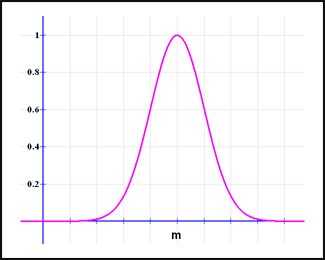
\includegraphics[width=.5\textwidth]{funcao_gaussiana}
  \caption[Gráfico da função de pertinência gaussiana]{Gráfico da função de pertinência gaussiana. Aqui a forma é de um sino, sendo que $\mu_A(x)$ é nula para todo $x \notin [m - \sigma, m + \sigma]$, crescente  até $altura(A)$, onde $x = m$ e decrescente até zero em $x = m + \sigma$.}
  % http://www.dma.fi.upm.es/recursos/aplicaciones/logica_borrosa/web/fuzzy_inferencia/funpert_en.htm
  \label{fig:funcao_fuzzy_gaussiana}
\end{figure}


%% ------------------------------------------------------------------------- %%
\subsection{Variáveis linguísticas}
\label{sec:variaveis_linguisticas}
Uma variável linguística é aquela cujo valor pode ser expresso por um termo qualitativo capaz de fornecer um significado conceitual à variável, tais como muito pequeno, pequeno, médio, baixo, alto e assim por diante, e que podem fornecer uma interpretação num contexto específico \citep{pedrycz:98}.

Para \citet{zadeh:75}, uma variável linguística é aquela cujo valor é uma palavra ou uma sentença numa linguagem natural ou artificial.

A motivação para o uso de variáveis linguísticas é que elas são, em geral, menos específicas do que variáveis numéricas \citep{zadeh:75}. Essa motivação tem um propósito particular quando os subconjuntos \emph{fuzzy} são determinados em termos de regras, já que o objetivo não é definir exaustivamente as variáveis linguísticas.

Cada variável linguística tem seus estados expressos por meio de termos de uma variável base, cujos valores são números reais dentro de um intervalo específico. Uma variável de base é uma variável no sentido clássico, por exemplo, temperatura, pressão, velocidade, tensão, umidade, idade, desempenho, salário, etc \citep{klir:95}.

Intuitivamente, as variáveis linguísticas  podem ser vistas como substantivos, por exemplo altura ou nota e os seus valores são adjetivos que caracterizam-nas, tais como alto, baixo, ruim, bom, dentre outros. A definição formal é dada em \ref{def:variavel_linguistica} \citep{zadeh:75, klir:95}.

% definição de variável linguística
\begin{defn}
\label{def:variavel_linguistica}
Uma variável linguística é caracterizada por uma quíntupla $(v, T, U, G, M)$, onde:

\begin{enumerate}[label=(\roman*)]
\item $v$ é o nome da variável.
\item $U$ é o universo de discurso.
\item $T$ é o conjunto de termos linguísticos de $v$ relacionado a uma variável base cujos valores variam ao longo de $U$.
\item $G$ é uma regra sintática, ou seja, a gramática para a geração de termos linguísticos em $T$.
\item $M$ é uma regra semântica que atribui para cada termo linguístico $t \in T$ seu significado, que é um conjunto \emph{fuzzy} em $U$.
\end{enumerate}
\end{defn}

\begin{exmp}
\textcolor{red}{Inserir um exemplo aqui da definição em \ref{def:variavel_linguistica}, de preferência linkada com o exemplo 2.1 e que faça sentido com o texto.}
\end{exmp}


%% ------------------------------------------------------------------------- %%
\subsection{Regras \emph{fuzzy}}\index{fuzzy!regras}
\label{sec:regras_fuzzy}
Os seres humanos tomam decisões baseados em regras, do tipo \emph{se} a temperatura está baixa, \emph{então} coloque um casaco, \emph{se} o combustível está acabando, \emph{então} abasteça o veículo, etc.

As regras estão entre as técnicas mais utilizadas para representar o conhecimento. Para \citet{zimmermann:01}, as regras ainda são amplamente utilizados devido ao fato de que tornam possível modelar o conhecimento em um sistema \emph{fuzzy} capturando-o por meio de especialistas. As regras também têm a vantagem de poderem ser expressas por uma linguagem natural ou artificial que, em geral, é facilmente compreensível.

De maneira similar a uma afirmação clássica, uma regra \emph{fuzzy} é composta por duas partes, resultando em uma estrutura do tipo \citep{dubois:96}:
\begin{center}
\emph{Se} \{antecedentes\}, \emph{então} \{consequentes\}.
\end{center}

Os antecedentes caracterizam premissas, enquanto a parte consequente são ações tomadas quando as premissas são atendidas. Diferentemente de uma regra clássica, um ou mais antecedentes podem ser parcialmente atendidos para que as premissas sejam aferidas e, portanto, as regras \emph{fuzzy} são mais relaxadas do que as regras clássicas que devem ser verificadas na sua totalidade.

A forma de interpretação mais comum e amplamente usada de uma regra \emph{fuzzy} é \citep{dubois:96}:
\begin{center}
\emph{Se} $x$ é $A$, \emph{então} $y$ é $B$.
\end{center}
\noindent onde $A$ e $B$ são variáveis linguísticas definidas por conjuntos \emph{fuzzy} em universos de discurso $U$ e $V$, respectivamente. Um exemplo da aplicação da regra pode ser visto em \ref{exp:regra_fuzzy}.

\begin{exmp}
\label{exp:regra_fuzzy}
\emph{Se} verde é baixo, \emph{então} pixel é pele.
\end{exmp}

É importante observar que \textbf{verde} é uma variável linguística e o adjetivo \textbf{baixo} é um termo linguístico representado como um número no intervalo $[0, 1]$ e, portanto, o antecedente é uma interpretação que retorna um único número desse intervalo. Por outro lado, a \textbf{pele} é a representação de um conjunto \emph{fuzzy} e, por isso, o consequente é uma atribuição de todo o conjunto \emph{fuzzy} $B$ para a variável de saída $y$, o pixel no exemplo \ref{exp:regra_fuzzy}. Porém, o consequente pode assumir outros valores que não só um conjunto \emph{fuzzy}, como também, um valor numérico clássico.

Também é válido destacar a possibilidade de utilizar conectivos na formação da regra para que ela seja estendida e tenha múltiplas partes, o que possibilita a interpretação de diversas variáveis linguísticas ao mesmo tempo em um contexto específico, como pode ser visto em \ref{exp:regra_fuzzy_mult}. Nesse caso, todas as partes dos antecedentes são calculadas simultaneamente em um único resultado, com base nos operadores destacados na seção \ref{sec:operacoes_conjuntos_fuzzy}.

\begin{exmp}
\label{exp:regra_fuzzy_mult}
\emph{Se} verde é médio e \emph{vermelho} é baixo e \emph{azul} é alto, \emph{então} pixel é não pele.
\end{exmp}

Apesar de ser possível empregar múltiplas partes também para os consequentes, tal capacidade não será utilizada e, consequentemente, não abordada neste trabalho.


%% ------------------------------------------------------------------------- %%
\section{Classificadores}
\label{sec:classificadores}
A aprendizagem de máquina é uma área que está preocupada com o desenvolvimento de programas de computador capazes de melhorar automaticamente com a experiência \citep{mitchell:97}. Essa definição está intimamente ligada ao modo com que seres humanos aprendem. Os esforços de pesquisa nessa área têm sido realizados com o propósito de aproximar esta relação.

Como exemplo, ao mostrar a imagem de uma árvore para uma criança de três anos de idade, muito provavelmente ela saberá reconhecê-la, pois deve ter sido exposta a situações em que tenha visto imagens semelhantes e, sendo assim, foi treinada para dar tal resposta. Logo, ela aprendeu o que é uma árvore apenas olhando para elas, não necessariamente por meio de definições matemáticas precisas. Em outras palavras, o aprendizado foi feito com base em dados que, muitas vezes, são utilizados para obter-se soluções empíricas para determinados problemas onde não há a possibilidade de se criar uma solução analítica \citep{mostafa:12}.

Analogamente, um algoritmo pode ser treinado para diferenciar uma árvore de outros objetos com base em um conjunto de dados que possui descrições sobre as árvores, tais como, altura, cores, espessura, comprimento, etc. Tais descrições também são chamadas de atributos, propriedades ou características e são submetidas a um classificador que avalia as evidências apresentadas e toma uma decisão sobre o objeto sendo analisado \citep{duda:12}. Essa tarefa começa com a definição de um vetor de características em um espaço $d$-dimensional, da forma \citep{duda:12}:

\begin{equation}
\label{eq:vetor_caracteristicas}
  x = 
  \begin{bmatrix}
    a_1 \\ a_2 \\ \vdots \\ a_d
  \end{bmatrix}
\end{equation}
\noindent onde $x \in X$ e $X$ é o espaço de entrada, ou seja, todos os $x$ vetores possíveis.

O conjunto de dados é formado por $N$ destes vetores e, sendo assim, o problema agora está em particionar o espaço de características de tal maneira que uma fronteira de decisão é formada \citep{duda:12}. Pode-se, então, atribuir uma classe ou rótulo $y$ específico para um dado vetor, onde $y \in Y$ e $Y$ é um conjunto finito de classes que, no caso binário, é da forma $Y = \{+1, -1\}$. A figura~\ref{fig:decision_boundary} mostra exemplos de particionamento de um espaço de características $2$-dimensional.

\begin{figure}[h]
    \centering
    \begin{minipage}{0.45\textwidth}
        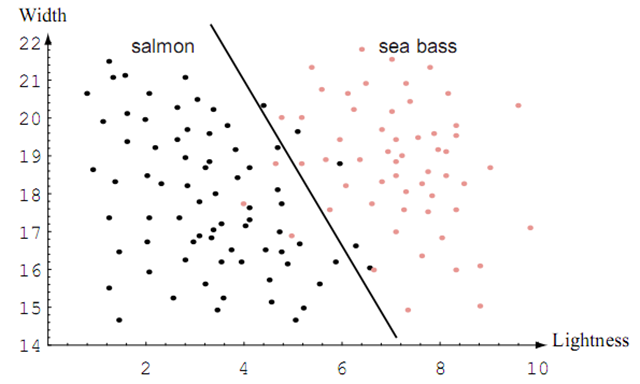
\includegraphics[width=\textwidth]{decision_boundary_linear}
        \label{fig:decision_boundary_linear}
    \end{minipage}
    ~ % space
    \begin{minipage}{0.45\textwidth}
        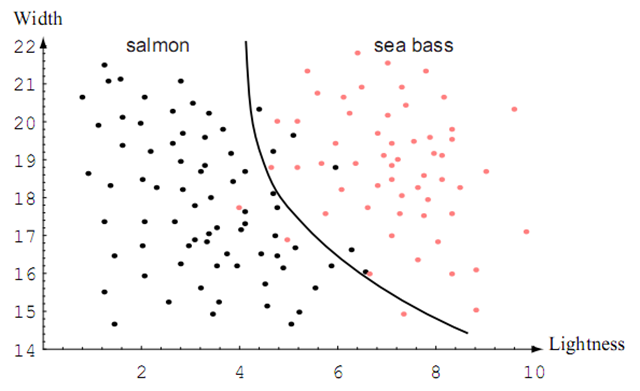
\includegraphics[width=\textwidth]{decision_boundary_smooth}
        \label{fig:decision_boundary_smooth}
    \end{minipage}
    \caption[Fronteira de decisão no espaço de características 2-dimensional]{Fronteira de decisão no espaço de características 2-dimensional. As figuras à esquerda e à direita representam a separação do espaço de características por funções linear e não linear, respectivamente. Vale ressaltar que, a complexidade computacional aumenta significativamente nos casos em que existem muitas características.\textcolor{red}{O ideal aqui é trocar essa distribuição pelo dataset de pele. A fonte dessas imagens é \citet{duda:12}}.}
    \label{fig:decision_boundary}
\end{figure}

Note que a fronteira de decisão é uma função hipotética que o algoritmo de aprendizado deve produzir com base no treinamento dos dados. Ela deve ser mais próxima possível de uma função alvo ou função objetivo $f : X\mapsto Y$ que é desconhecida \citep{mostafa:12}.

Este tipo de abordagem é caracterizada como aprendizagem supervisionada, ou seja, os dados de treinamento contêm amostras explícitas de como deve ser a saída correta sobre um vetor de entrada \citep{mostafa:12}.

Na aprendizagem não supervisionada, também conhecida como clusterização, não se sabe a que classes pertencem os dados de treinamento. A missão do classificador, neste caso, é aglomerar os dados de entrada em agrupamentos naturais \citep{duda:12}. Logo, a aprendizagem não supervisionada pode ser vista como uma tarefa de encontrar padrões ou estruturas espontaneamente a partir dos dados de entrada \citep{mostafa:12}.

Uma outra abordagem é a aprendizagem reforçada que, da mesma forma que na aprendizagem não supervisionada, não usa dados de entrada rotulados, em vez disso, a saída proposta pelo treinamento é utilizada juntamente com uma medida de sua qualidade para melhorar os resultados do classificador \citep{mostafa:12}.

Ainda sobre os resultados do classificador, é importante salientar que aprender os parâmetros de uma função alvo e testá-la nos mesmos dados é um erro fundamental, pois o modelo repetiria os rótulos das amostras tão logo treinadas implicando em um ajuste perfeito dos dados, porém, não seria suficiente para prever qualquer coisa útil sobre novos dados de entrada. Esta situação é chamada de \emph{overfitting} e para evitá-la, o conjunto de dados é, então, particionado de forma a armazenar parte dos dados para uma etapa subsequente de teste, no intuito de encontrar o estimador com a melhor performance \citep{mostafa:12}.

A divisão dos dados em subconjuntos disjuntos de treinamento e de teste é uma abordagem eficaz quando uma grande quantidade de dados está disponível. Entretanto, quando os dados são limitados, a retenção de parte deles para o conjunto de teste reduz ainda mais o número de amostras disponíveis para treinamento \citep{mitchell:97}. Logo, uma outra abordagem, conhecida como validação cruzada, pode ser aplicada de modo que todo o conjunto de dados é usado no treinamento e teste.

A validação cruzada\index{cruzada!validação} consiste em dividir o conjunto de dados $D$ em $K$ subconjuntos disjuntos $D_1, D_2, \ldots, D_K$, onde cada subconjunto tem tamanho aproximado $N/K$. O modelo é, então, treinado em cada um desses subconjuntos, exceto um que é mantido como um conjunto de validação, no qual a medida de erro é realizada. Este processo é repetido $K$ vezes, de tal forma que cada um dos subconjuntos tem a oportunidade de agir como o conjunto de teste e, por isso, essa abordagem também é conhecida como \emph{K-fold}. Ao final de todas as $K$ iterações, a média do erro obtido por cada estimador é usado como a medida de performance do classificador \citep{mostafa:12}.

Alguns dos classificadores, que foram usados nos experimentos preliminares do capítulo \ref{cap:experimentos}, serão brevemente tratados nas seções \ref{sec:clasificadores_svm} e \ref{sec:clasificadores_knn}.


%% ------------------------------------------------------------------------- %%
\subsection{Máquinas de vetores suporte}
\label{sec:clasificadores_svm}
As Máquinas de Vetores Suporte (SVM) constituem uma técnica de aprendizagem computacional baseada na Teoria de Aprendizado Estatístico \citep{vapnik:13}, cujo objetivo era de resolver problemas de classificação de padrões. Na prática, uma SVM tem a habilidade de gerar um hiperplano ou conjunto de hiperplanos num espaço de alta ou infinita dimensionalidade, que pode ser usado para tarefas de classificação, regressão ou outras \citep{duda:12}.

Derivado do próprio nome da técnica, os vetores de suporte são as amostras do conjunto de treinamento que definem o hiperplano ótimo e são os padrões mais difíceis de classificar \citep{duda:12}. Intuitivamente, eles são os padrões mais relevantes para a tarefa de classificação, pois uma mudança nestes vetores implicam diretamente no resultado do hiperplano ótimo \footnote{O hiperplano de separação ótimo de uma SVM é aquele de uma classe de hiperplanos com a maior margem de separação entre os dois conjuntos de treinamento \citep{cortes:95}.}.

Seja o conjunto de dados de treinamento com $N$ amostras da forma:
\begin{equation}
\label{eq:svm_dataset}
    D = (x_1, y_1), (x_2, y_2), \ldots, (x_N, y_N)
\end{equation}
\noindent onde cada $x_i$ é um vetor $d$-dimensional da forma dada em \ref{eq:vetor_caracteristicas}, $i = 1, 2, \ldots, N$, $y_i \in Y$ e $Y = \{+1, -1\}$. Portanto, o conjunto de treinamento contém $N$ observações com suas respectivas classes.

Assumindo que $D$ é linearmente separável, pode-se separar os dados por meio de um hiperplano usando um classificador, também linear, definido pela equação \citep{lorena:03}:
\begin{equation}
\label{eq:svm_hyperplano_otimo}
w \cdot x + b = 0
\end{equation}
\noindent onde $w \cdot x$ é um produto escalar, $w$ é o vetor normal ao hiperplano e $b$ é um termo compensador. O parâmetro $\ffrac{b}{||w||}$ determina o deslocamento do hiperplano em relação à origem.

A partir dessa definição, outros dois hiperplanos paralelos ao hiperplano ótimo podem ser obtidos, conforme as equações em \ref{eq:svm_hyperplanos_paralelos}, de forma que uma região delimitada, conhecida como margem, se forma entre eles.

\begin{equation}
\label{eq:svm_hyperplanos_paralelos}
\begin{cases}
    w \cdot x + b = +1\\
    w \cdot x + b = -1
\end{cases}
\end{equation}

Além disso, algumas restrições são definidas para evitar que não existam pontos entre $w \cdot x + b = 0$ e $w \cdot x + b = \pm 1$, formalmente tem-se \citep{lorena:03}:
\begin{equation}
\label{eq:svm_hyperplanos_paralelos_restricoes}
\begin{cases}
    w \cdot x_i + b \geq +1, & \text{se}\ y_i = +1\\
    w \cdot x_i + b \leq -1, & \text{se}\ y_i = -1
\end{cases}
\end{equation}
\noindent ou, equivalentemente:
\begin{equation}
\label{eq:svm_hyperplanos_paralelos_restricoes_equiv}
    y_i (w \cdot x_i + b) \geq 1
\end{equation}

Segundo \citet{campbell:00}, no sistema dado na equação \ref{eq:svm_hyperplanos_paralelos_restricoes}, supõe-se que a margem é sempre maior que a distância entre $w \cdot x + b = 0$ e $|w \cdot x + b = 1|$ e, por essa razão, SVMs desta natureza são usualmente denominadas de SVMs com margens rígidas. A figura~\ref{fig:svm_support_vectors} mostra a representação gráfica destes conceitos.

\begin{figure}[!h]
  \centering
  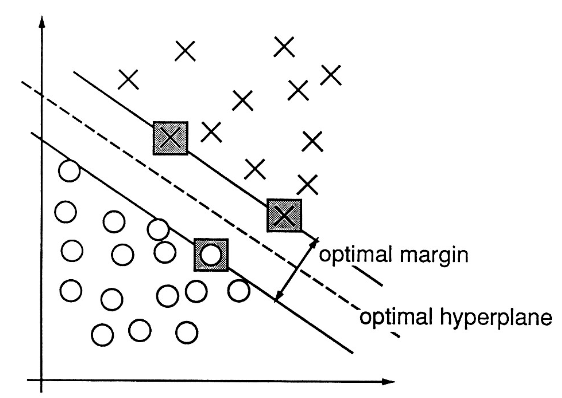
\includegraphics[width=.5\textwidth]{svm_support_vectors}
  \caption[Exemplo de um problema de classes binárias separáveis num espaço $2$-dimensional]{Exemplo de um problema de classes binárias separáveis num espaço $2$-dimensional. Os vetores de suporte, marcados com quadrados cinza, definem a margem de maior separação entre as duas classes. \textcolor{red}{Aqui também é interessante colocar as amostras de pele e não pele, talvez somente com duas características. Essa imagem é de \citep{cortes:95}}}
  \label{fig:svm_support_vectors}
\end{figure}

Geometricamente, a distância entre os dois hiperplanos paralelos ao hiperplano ótimo é $\ffrac{2}{||w||}$. Consequentemente, pode-se deduzir que a distância entre o hiperplano ótimo e $w \cdot x + b = \pm 1$ é $\ffrac{1}{||w||}$. Portanto, a minimização de $||w||$ maximiza a margem e, sendo assim, tem-se um problema de otimização no qual deseja-se minimizar $||w||^2$ sujeito às restrições em \ref{eq:svm_hyperplanos_paralelos_restricoes_equiv} \citep{lorena:03}. Logo, $w$ e $b$ ótimos que resolvem este problema definem o classificador e podem ser obtidos por multiplicadores de Lagrange \citep{campbell:00}:
\begin{equation}
\label{eq:svm_margens_rigidas}
\text{Maximizar: } \sum_{i=1}^N \alpha_i - \frac{1}{2} \sum_{i, j=1}^N \alpha_i \alpha_j y_i y_j x_i\cdot x_j
\end{equation}

\begin{equation}
\label{eq:svm_margens_rigidas_restricoes}
\text{Sujeito a: }
\begin{cases}
    \alpha_i \geq 0\\[1em]
    \sum_{i=1}^N \alpha_i y_i = 0
\end{cases}
\end{equation}
\noindent onde $\alpha$ são os multiplicadores de Lagrange.

É importante ressaltar que este tipo de SVM tem êxito em conjuntos de dados de treinamento linearmente separáveis. Nos casos em que os dados são não linearmente separáveis, é admitida a ocorrência de alguns erros de classificação para o conjunto de treinamento, pela inclusão de variáveis de relaxamento \citep{lorena:03}. Essas alterações foram produzidas por \citet{cortes:95} e fazem parte de uma técnica denominada suavização de margens e, por conseguinte, SVMs dessa família também são chamadas de SVM com margens suaves. Logo, o problema de otimização torna-se \citep{lorena:03}:
\begin{equation}
\label{eq:svm_margens_suaves_def}
\text{Minimizar: } ||w||^2 + C\sum_{i=1}^N \xi_i
\end{equation}

\begin{equation}
\label{eq:svm_margens_suaves_def_restricoes}
\text{Sujeito a: }
\begin{cases}
    \xi_i \geq 0\\[1em]
    y_i (w \cdot x_i + b) \geq 1 - \xi_i
\end{cases}
\end{equation}
\noindent onde $C$ é uma constante de regularização determinada empiricamente que impõe um peso diferente para o treinamento em relação à generalização. Sendo assim, o problema pode ser resolvido da mesma maneira com a equação em \ref{eq:svm_margens_rigidas}, porém, com algumas alterações nas restrições \citep{lorena:03}:

\begin{equation}
\label{eq:svm_margens_suaves_restricoes}
\text{Sujeito a: }
\begin{cases}
    0 \leq \alpha_i \leq C\\[1em]
    \sum_{i=1}^N \alpha_i y_i = 0
\end{cases}
\end{equation}

Em geral, a maioria dos problemas de classificação impedem que classificadores lineares sejam utilizados por não ser possível obter resultados satisfatórios na partição dos dados de treinamento por um hiperplano. Entretanto, as SVMs lineares podem ser estendidas para lidar com essa situação mapeando o espaço de entrada em um espaço de características de dimensão mais alta, tipicamente muito maior que o espaço original \citep{duda:12}, da forma:
\begin{equation}
\label{eq:svm_dataset_transformado}
    D' = (\Phi(x_1), y_1), (\Phi(x_2), y_2), \ldots, (\Phi(x_N), y_N)
\end{equation}

A escolha apropriada de uma função $\Phi$ torna o conjunto de treinamento linearmente separável no espaço transformado \citep{lorena:03}. A forma do hiperplano ótimo agora é definida por:
\begin{equation}
\label{eq:svm_hyperplano_otimo_trasnformado}
w \cdot \Phi(x) + b = 0
\end{equation}

Logo, os conceitos de vetores de suporte, margem, hiperplanos paralelos e, consequentemente, de problema de otimização para encontrar a solução para os parâmetros $w$ e $b$ se aplicam aqui de forma similar. Formalmente, o problema de otimização pode ser resolvido como \citep{lorena:03}:
\begin{equation}
\label{eq:svm_nao_linear}
\text{Maximizar: } \sum_{i=1}^N \alpha_i - \frac{1}{2} \sum_{i, j=1}^N \alpha_i \alpha_j y_i y_j \Phi(x_i)\cdot \Phi(x_j)
\end{equation}
\noindent sujeito às mesmas restrições definidas em \ref{eq:svm_margens_suaves_restricoes}.

Agora, há a necessidade de se definir como o produto interno $\Phi(x_i)\cdot \Phi(x_j)$ entre dois vetores quaisquer $x_i, x_j \in D$ é realizado, cuja resposta está na introdução do conceito de \emph{kernels} \citep{lorena:03}.

\emph{Kernels} são funções\index{\emph{kernel}!funções} que têm a finalidade de projetar os vetores de entrada num espaço de características com número de dimensões exponencial ou infinito \citep{taylor:04}, da forma:
\begin{equation}
\label{eq:svm_kernels}
k(x_i, x_j) =  \Phi(x_i) \cdot \Phi(x_j)
\end{equation}

Logo, é possível aplicar um \emph{kernel} como descrito na equação \ref{eq:svm_kernels} na etapa de otimização da SVM, calculando de maneira eficiente o produto interno a partir dos dados de entrada, sem nem mesmo computar explicitamente o mapeamento da função $\Phi$ \citep{taylor:04}.

Alguns dos \emph{kernels} mais utilizados são \citep{lorena:03}:
\begin{enumerate}[label=(\roman*)]
\item \emph{Kernel} linear\index{\emph{kernel}!linear}
\begin{equation}
\label{eq:svm_kernel_linear}
k(x_i, x_j) =  (x_i \cdot x_j)
\end{equation}
O \emph{kernel} linear é o mais simples das funções \emph{kernel} e se dá pelo produto interno de dois vetores $x_i$ e $x_j$.

\item \emph{Kernel} polinomial\index{\emph{kernel}!polinomial}
\begin{equation}
\label{eq:svm_kernel_polinomial}
k(x_i, x_j) =  ({\gamma x_i \cdot y_i + r} )^g
\end{equation}
\noindent onde $g$ é o grau do polinômio e $r$ é um termo constante. Para este \emph{kernel}, os mapeamentos $\Phi$ também são funções polinomiais e, portanto, a complexidade é proporcional à escolha de $g$ \citep{lorena:03}.

\item \emph{Kernel} gaussiano\index{\emph{kernel}!gaussiano ou RBF}
\begin{equation}
\label{eq:svm_kernel_rbf}
k(x_i, x_j) =  \exp{\big(-\gamma {||x_i - y_i||}^2 \big)}
\end{equation}
Também conhecido como Função de Base Radial (RBF), o \emph{kernel} gaussiano corresponde a um espaço de características de dimensão infinita \citep{lorena:03}.
\end{enumerate}

No \emph{kernel} RBF e polinomial, o parâmetro $\gamma$ pode ser visto como o inverso do raio de influência das amostras selecionadas pelo modelo como vetores de suporte \citep{scikit-learn:11}.

%% ------------------------------------------------------------------------- %%
\subsection{\emph{k}-vizinhos mais próximos}
\label{sec:clasificadores_knn}
O $k$-Vizinhos Mais Próximos ($k$-NN) é um algoritmo baseado em instâncias, o que significa que a função alvo não é aprendida com base em amostras de treinamento; elas simplesmente são mantidas, de maneira que a relação entre uma nova amostra com as amostras de treinamento armazenadas é avaliada e uma função alvo é, então, atribuída a ela \citep{mitchell:97}.

Como o próprio nome sugere, o $k$-NN classifica um novo ponto $x$ atribuindo-lhe a classe de maior frequência dentre as $k$ amostras mais próximas, ou seja, a decisão da classe de $x$ é feita por maioria de votos dos $k$ vizinhos mais próximos e, por essa razão, é interessante que a escolha de $k$ seja um número ímpar para evitar empates \citep{duda:12}.

\begin{figure}[!h]
  \centering
  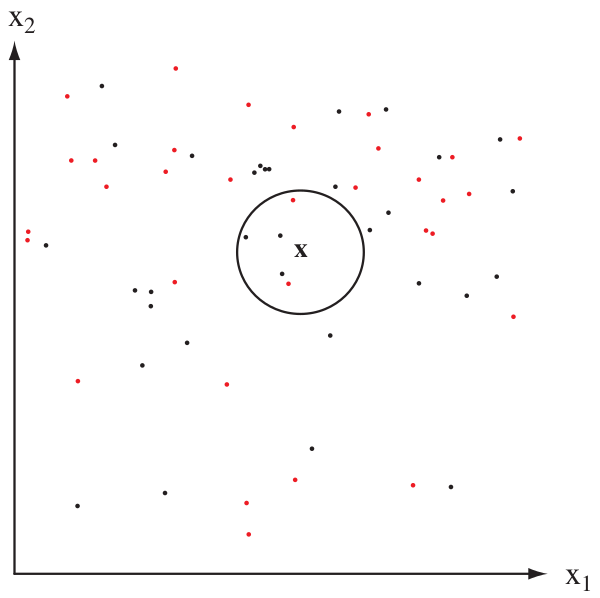
\includegraphics[width=.45\textwidth]{knn_exemplo}
  \caption[Exemplo de aplicação do $k$-NN na tarefa de classificação em um espaço $2$-dimensional]{Exemplo de aplicação do k-NN na tarefa de classificação em um espaço $2$-dimensional. O algoritmo avalia as $k$ amostras próximas de $x$, criando uma região esférica, e rotula $x$ com a classe de maior frequência. Neste caso, $k = 5$ e a classe atribuída a $x$ deve ser a mesma dos pontos em preto. \textcolor{red}{Aqui também é interessante colocar as amostras de pele e não pele, talvez somente com duas características. Essa imagem é de \citep{duda:12}}}
  \label{fig:knn_exemplo}
\end{figure}

Seja $D$ o conjunto de dados de treinamento com $N$ amostras da forma apresentada em \ref{eq:svm_dataset}. Logo, a distância entre duas amostras $x_i$ e $x_j$ quaisquer pode ser obtida em termos da distância Euclidiana, definida como:

\begin{equation}
\label{eq:knn_distancia_euclidiana}
d(x_i, x_j) = \sqrt{\sum_{r=1}^d (a_r(x_i) - a_r(x_j))^2}
\end{equation}
\noindent onde $a_r$ refere-se ao $r$-ésimo atributo do vetor de entrada $x$ e $i, j = 1, 2, \ldots, N$. Outras métricas de distância podem ser atribuídas a $d(x_i, x_j)$, tais como, Manhattan, Chebyshev e Minkowski \citep{duda:12}.

Para, então, classificar uma nova amostra $x_q$, toma-se $x_1, \ldots, x_k$ instâncias do conjunto de treinamento, cujas distâncias dadas por \ref{eq:knn_distancia_euclidiana}, são dos $k$ pontos mais próximos de $x_q$. Sendo assim, a função que estima a classe de $x_q$ é dada por \citep{mitchell:97}:
\begin{equation}
\label{eq:knn_funcao_argmax}
g(x_q) \gets \argmax_{y \in Y} \sum_{i=1}^k \delta (y, f(x_i))
\end{equation}
\noindent onde
\begin{equation}
\label{eq:knn_delta}
  \delta (y, f(x_i)) =  \begin{cases}
                1, \quad \text{se}\ y = f(x_i) \\
                0, \quad \text{caso contrário}
              \end{cases}
\end{equation}

É importante ressaltar que $f(x_i)$ é conhecida, ou seja, é a classe da amostra $x_i$ do conjunto de treinamento.

Uma variação óbvia da função dada na equação \ref{eq:knn_funcao_argmax} é a atribuição de pesos de cada um dos $k$ vizinhos, conforme sua distância, para um ponto $x_q$ sendo classificado \citep{mitchell:97}. Essa variação implica que pontos mais próximos de $x_q$ têm maior influência na sua rotulação. Formalmente, tem-se que \citep{mitchell:97}:
\begin{equation}
\label{eq:knn_funcao_argmax_pesos}
g(x_q) \gets \argmax_{y \in Y} \sum_{i=1}^k w_i \delta (y, f(x_i))
\end{equation}
\noindent onde
\begin{equation}
\label{eq:knn_funcao_peso}
  w_i = \frac{1}{d(x_q, x_i)^2}
\end{equation}

No caso em que $d(x_q, x_i) = 0$, ou seja, $x_q$ e $x_i$ estão exatamente nas mesmas coordenadas, $g(x_q)$ pode assumir o mesmo valor de $f(x_i)$. Se há outras amostras de treinamento $x_i$ com a mesma característica, então $x_q$ pode assumir a classe da maioria delas \citep{mitchell:97}.


%% ------------------------------------------------------------------------- %%
\subsection{Árvores de decisão}
\label{sec:clasificadores_arvores_decisao}
Árvore de decisão é um método para aproximação de funções alvo discretas, nas quais a função aprendida é representada por uma árvore de decisão ou, ainda, por um conjunto de regras do tipo \emph{Se-Então} que são de fácil interpretação. É uma das técnicas de aprendizagem mais populares de inferência indutiva\footnote{A tarefa de indução é desenvolver uma regra de classificação que pode determinar a classe de qualquer objeto a partir dos valores de seus atributos \citep{quinlan:86}.} \citep{mitchell:97}.

As amostras de um conjunto de dados são classificadas por uma árvore de decisão por um processo iterativo onde um atributo (nó) é escolhido como raiz até algum nó folha, onde a classe é atribuída à amostra. Cada ramo partindo de um nó representa um dos valores possíveis de um dado atributo \citep{mitchell:97}.

Há uma família de algoritmos de árvore de decisão. Um deles é o Divisor Iterativo 3 (ID3) proposto por \citet{quinlan:86}. O ID3 avalia cada atributo através de um teste estatístico para determinar o quão bem ele, por si só, classifica as amostras de treinamento. O melhor atributo é selecionado como o nó raiz da árvore. Um ramo descendente do nó raiz é criado para cada valor possível deste atributo e as amostras de treinamento são classificadas para o nó descendente adequado. Este processo é então repetido recursivamente utilizando as amostras associadas a cada nó descendente. Esse é um algoritmo de busca guloso, já que ele não retrocede para reconsiderar escolhas anteriores \citep{mitchell:97}. O algoritmo para quando o subconjunto de amostras associado a um nó é da mesma classe ou quando não há relevância estatística para uma nova partição \citep{quinlan:86}.

Para medir a impureza de uma partição, o ID3 usa o conceito de entropia, formalmente \citep{quinlan:86}:

\begin{equation}
\label{eq:arvore_devisao_entropia}
H(D) = - y_\oplus log_2 y_\oplus - y_\ominus log_2 y_\ominus
\end{equation}
\noindent onde $D$ é o conjunto de dados de treinamento com $N$ amostras da forma apresentada em \ref{eq:svm_dataset}, $y_\oplus$ e $y_\ominus$ é a proporção de amostras positivas e negativas de $D$, respectivamente. É importante notar que a entropia é 0 quando todas as amostras de $D$ pertencem à mesma classe, 1 quando $D$ contém um número igual de amostras positivas e negativas e um valor entre 0 e 1 nos demais casos \citep{mitchell:97}.

Dada a entropia como uma medida de impureza de um conjunto de amostras de treinamento, pode-se definir o teste estatístico, conhecido como ganho de informação, que mede a efetividade de um atributo na classificação dos dados de treinamento, formalmente \citep{quinlan:86}:
\begin{equation}
\label{eq:arvore_devisao_ganho_informacao}
IG(D, a_r) = H(D) - \sum_{v \in V(a_r)} \frac{|D_v|}{|D|} H(D_v)
\end{equation}
\noindent onde $V(a_r)$ é o conjunto de todos os possíveis valores do atributo $a_r$, $D_v$ é o subconjunto de $D$ no qual o atributo $a_r$ tem o valor $v$.

Vale enfatizar que o primeiro termo da equação dado em \ref{eq:arvore_devisao_ganho_informacao} é a entropia do conjunto original $D$ e o segundo termo é o valor esperado da entropia depois que $D$ é particionado usando o atributo $a_r$ \citep{mitchell:97}. Outro aspecto importante é que o algoritmo inicia com o conjunto $D$ original, que é substituído por $D_v$ à medida que a recursão se aprofunda.

Batizado de C4.5, \citet{quinlan:93} estendeu o ID3 para possibilitar o uso de atributos contínuos, atributos com dados ausentes e melhoria na eficiência computacional. Além disso, essa versão cuida de questões como quão profunda a árvore deve ser para evitar que os dados de treinamento sejam perfeitamente classificados, ou seja, quando o conjunto de treinamento é particionado até que cada subconjunto contenha apenas amostras de uma única classe. A estratégia adotada por \citet{quinlan:93} foi podar a árvore posteriormente à geração da árvore ajustada. Esse processo, apesar de ser mais lento que a proposta anterior do ID3, tornou o algoritmo mais confiável e com maior capacidade de generalização.


%% ------------------------------------------------------------------------- %%
\begin{comment}
\section{Exemplo de Código-Fonte em Java}
\label{sec:exemplo_codigo_fonte}
% Foi utilizado o pacote listing para formatar código fonte
% http://ctan.org/tex-archive/macros/latex/contrib/listings/listings.pdf
% Veja no preambulo do arquivo tese-exemplo.tex os parâmetros de configuração.

\begin{lstlisting}[frame=trbl]
   for(i = 0; i < 20; i++)
   {
       // Comentário 
       System.out.println("Mensagem...");
   }
\end{lstlisting}
\end{comment}
